% !TeX spellcheck = en-US
% !TeX encoding = utf8
% !TeX program = pdflatex
% !BIB program = biber
% -*- coding:utf-8 mod:LaTeX -*-


% vv  scroll down to line 200 for content  vv


\let\ifdeutsch\iffalse
\let\ifenglisch\iftrue
% EN: This file is loaded before the \documentclass command in the main document

% EN: The following package allows \\ at the title page
%     For more information see https://github.com/latextemplates/scientific-thesis-cover/issues/4
\RequirePackage{kvoptions-patch}

\ifenglisch
  \PassOptionsToClass{numbers=noenddot}{scrbook}
\else
  %()Aus scrguide.pdf - der Dokumentation von KOMA-Script)
  %Nach DUDEN steht in Gliederungen, in denen ausschließlich arabische Ziffern für die Nummerierung
  %verwendet werden, am Ende der Gliederungsnummern kein abschließender Punkt
  %(siehe [DUD96, R3]). Wird hingegen innerhalb der Gliederung auch mit römischen Zahlen
  %oder Groß- oder Kleinbuchstaben gearbeitet, so steht am Ende aller Gliederungsnummern ein
  %abschließender Punkt (siehe [DUD96, R4])
  \PassOptionsToClass{numbers=autoendperiod}{scrbook}
\fi

% Warns about outdated packages and missing caption declarations
% See https://www.ctan.org/pkg/nag
\RequirePackage[l2tabu, orthodox]{nag}

%DE: Neue deutsche Trennmuster
%    Siehe http://www.ctan.org/pkg/dehyph-exptl und http://projekte.dante.de/Trennmuster/WebHome
%    Nur für pdflatex, nicht für lualatex
\RequirePackage{ifluatex}
\ifluatex
  % do not load anything
\else
  \ifdeutsch
    \RequirePackage[ngerman=ngerman-x-latest]{hyphsubst}
  \fi
\fi

\documentclass[
  % fontsize=11pt is the standard
  a4paper,  % Standard format - only KOMAScript uses paper=a4 - https://tex.stackexchange.com/a/61044/9075
  twoside,  % we are optimizing for both screen and two-sided printing. So the page numbers will jump, but the content is configured to stay in the middle (by using the geometry package)
  bibliography=totoc,
  %               idxtotoc,   %Index ins Inhaltsverzeichnis
  %               liststotoc, %List of X ins Inhaltsverzeichnis, mit liststotocnumbered werden die Abbildungsverzeichnisse nummeriert
  headsepline,
  cleardoublepage=empty,
  parskip=half,
  %               draft    % um zu sehen, wo noch nachgebessert werden muss - wichtig, da Bindungskorrektur mit drin
  draft=false
]{scrbook}
% !TeX encoding = utf8
% -*- coding:utf-8 mod:LaTeX -*-

% EN: This file includes basic packages and sets options. The order of package
%     loading is important

% DE: In dieser Datei werden zuerst die benoetigten Pakete eingebunden und
%     danach diverse Optionen gesetzt. Achtung Reihenfolge ist entscheidend!


% EN: Styleguide:
% - English comments are prefixed with "EN", German comments are prefixed with "DE"
% - Prefixed headings define the language for the subsequent paragraphs
% - It is tried to organize packages in blocks. Bocks are separated by two empty lines.

% DE: Styleguide:
%
% Ein sehr kleiner Styleguide. Packages werden in Blöcken organisiert.
% Zwischen zwei Blöcken sind 2 Leerzeilen!


% EN: Enable copy and paste of text from the PDF
%     Only required for pdflatex. It "just works" in the case of lualatex.
%     mmap enables mathematical symbols but does not work with the newtx font set
%     See: https://tex.stackexchange.com/a/64457/9075
%     Other solutions outlined at http://goemonx.blogspot.de/2012/01/pdflatex-ligaturen-und-copynpaste.html and http://tex.stackexchange.com/questions/4397/make-ligatures-in-linux-libertine-copyable-and-searchable
%     Troubleshooting outlined at https://tex.stackexchange.com/a/100618/9075

\ifluatex
\else
  \usepackage{cmap}
\fi


% EN: File encoding
% DE: Codierung
%     Wir sind im 21 Jahrhundert, utf-8 löst so viele Probleme.
%
% Mit UTF-8 funktionieren folgende Pakete nicht mehr. Bitte beachten!
%   * fancyvrb mit §
%   * easylist -> http://www.ctan.org/tex-archive/macros/latex/contrib/easylist/
\ifluatex
  % EN: See https://tex.stackexchange.com/a/158517/9075
  %     Not required, because of usage of fontspec package
  %\usepackage[utf8]{luainputenc}
\else
  \usepackage[utf8]{inputenc}
\fi


% DE: Parallelbetrieb tex4ht und pdflatex

\makeatletter
\@ifpackageloaded{tex4ht}{
  \def\iftex4ht{\iftrue}
}{
  \def\iftex4ht{\iffalse}
}
\makeatother


% EN: Mathematics
% DE: Mathematik
%
% DE: Viele Mathematik-Sachen. Siehe https://texdoc.net/pkg/amsmath
%
% EN: Options must be passed this way, otherwise it does not work with glossaries
% DE: fleqn (=Gleichungen linksbündig platzieren) funktioniert nicht direkt. Es muss noch ein Patch gemacht werden:
\PassOptionsToPackage{fleqn,leqno}{amsmath}
%
% DE: amsmath Muss nicht mehr geladen werden, da es von newtxmath automatisch geladen wird
% \usepackage{amsmath}


%% EN: Fonts
%% DE: Schriften
%%
%% !!! If you change the font, be sure that words such as "workflow" can
%% !!! still be copied from the PDF. If this is not the case, you have
%% !!! to use glyphtounicode. See comment at cmap package


% EN: Times Roman for all text
\ifluatex
  \RequirePackage{amsmath}
  \RequirePackage{unicode-math}
  \setmainfont{TeX Gyre Termes}
  \setmathfont{texgyretermes-math.otf}
  \setsansfont[Scale=.9]{TeX Gyre Heros}
  \setmonofont[StylisticSet={1,3},Scale=.9]{inconsolata}
\else
  \RequirePackage{newtxtext}
  \RequirePackage{newtxmath}
  % EN: looks good with times, but no equivalent for lualatex found,
  %     therefore replaced with inconsolata
  %\RequirePackage[zerostyle=b,scaled=.9]{newtxtt}
  \RequirePackage[varl,scaled=.9]{inconsolata}

  % DE: Symbole
  % unicode-math scheint für die meisten schon etwas anzubieten
  %
  %\usepackage[geometry]{ifsym} % \BigSquare

  % EN: The euro sign
  % DE: Das Euro Zeichen
  %     Fuer Palatino (mathpazo.sty): richtiges Euro-Zeichen
  %     Alternative: \usepackage{eurosym}
  \newcommand{\EUR}{\ppleuro}
\fi


% DE: Noch mehr Symbole
%\usepackage{stmaryrd} %fuer \ovee, \owedge, \otimes
%\usepackage{marvosym} %fuer \Writinghand %patched to not redefine \Rightarrow
%\usepackage{mathrsfs} %mittels \mathscr{} schoenen geschwungenen Buchstaben erzeugen
%\usepackage{calrsfs} %\mathcal{} ein bisserl dickeren buchstaben erzeugen - sieht net so gut aus.

% EN: Fallback font - if the subsequent font packages do not define a font (e.g., monospaced)
%     This is the modern package for "Computer Modern".
%     In case this gets activated, one has to switch from cmap package to glyphtounicode (in the case of pdflatex)
% DE: Fallback-Schriftart
%\usepackage[%
%    rm={oldstyle=false,proportional=true},%
%    sf={oldstyle=false,proportional=true},%
%    tt={oldstyle=false,proportional=true,variable=true},%
%    qt=false%
%]{cfr-lm}

% EN: Headings are typset in Helvetica (which is similar to Arial)
% DE: Schriftart fuer die Ueberschriften - ueberschreibt lmodern
%\usepackage[scaled=.95]{helvet}

% DE: Für Schreibschrift würde tun, muss aber nicht
%\usepackage{mathrsfs} %  \mathscr{ABC}

% EN: Font for the main text
% DE: Schriftart fuer den Fliesstext - ueberschreibt lmodern
%     Linux Libertine, siehe http://www.linuxlibertine.org/
%     Packageparamter [osf] = Minuskel-Ziffern
%     rm = libertine im Brottext, Linux Biolinum NICHT als serifenlose Schrift, sondern helvet (von oben) beibehalten
%\usepackage[rm]{libertine}

% EN: Alternative Font: Palantino. It is recommended by Prof. Ludewig for German texts
% DE: Alternative Schriftart: Palantino, Packageparamter [osf] = Minuskel-Ziffern
%     Bitte nur in deutschen Texten
%\usepackage{mathpazo} %ftp://ftp.dante.de/tex-archive/fonts/mathpazo/ - Tipp aus DE-TEX-FAQ 8.2.1

% DE: Schriftart fuer Programmcode - ueberschreibt lmodern
%     Falls auskommentiert, wird die Standardschriftart lmodern genommen
%     Fuer schreibmaschinenartige Schluesselwoerter in den Listings - geht bei alten Installationen nicht, da einige Fontshapes (<>=) fehlen
%\usepackage[scaled=.92]{luximono}
%\usepackage{courier}
% DE: BeraMono als Typewriter-Schrift, Tipp von http://tex.stackexchange.com/a/71346/9075
%\usepackage[scaled=0.83]{beramono}

% EN: backticks (`) are rendered as such in verbatim environments.
%     See the following links for details:
%     - https://tex.stackexchange.com/a/341057/9075
%     - https://tex.stackexchange.com/a/47451/9075
%     - https://tex.stackexchange.com/a/166791/9075
\usepackage{upquote}

% EN: For \texttrademark{}
\usepackage{textcomp}

% EN: name-clashes von marvosym und mathabx vermeiden:
\def\delsym#1{%
  %  \expandafter\let\expandafter\origsym\expandafter=\csname#1\endcsname
  %  \expandafter\let\csname orig#1\endcsname=\origsym
  \expandafter\let\csname#1\endcsname=\relax
}

%\usepackage{pifont}
%\usepackage{bbding}
%\delsym{Asterisk}
%\delsym{Sun}\delsym{Mercury}\delsym{Venus}\delsym{Earth}\delsym{Mars}
%\delsym{Jupiter}\delsym{Saturn}\delsym{Uranus}\delsym{Neptune}
%\delsym{Pluto}\delsym{Aries}\delsym{Taurus}\delsym{Gemini}
%\delsym{Rightarrow}
%\usepackage{mathabx} - Ueberschreibt leider zu viel - und die \le-Zeichen usw. sehen nicht gut aus!


% EN: Modern font encoding
%     Has to be loaded AFTER any font packages. See https://tex.stackexchange.com/a/2869/9075.
\ifluatex
\else
  \usepackage[T1]{fontenc}
\fi
%


% EN: Character protrusion and font expansion. See http://www.ctan.org/tex-archive/macros/latex/contrib/microtype/
% DE: Optischer Randausgleich und Grauwertkorrektur

\usepackage[
  babel=true, % EN: Enable language-specific kerning. Take language-settings from the language of the current document (see Section 6 of microtype.pdf)
  expansion=alltext,
  protrusion=alltext-nott, % EN: Ensure that at listings, there is no change at the margin of the listing
  final % EN: Always enable microtype, even if in draft mode. This helps finding bad boxes quickly.
        %     In the standard configuration, this template is always in the final mode, so this option only makes a difference if "pros" use the draft mode
]{microtype}


% EN: \texttt{test -- test} keeps the "--" as "--" (and does not convert it to an en dash)
\DisableLigatures{encoding = T1, family = tt* }

% DE: fuer microtype
% DE: tracking=true muss als Parameter des microtype-packages mitgegeben werden
% DE: Deaktiviert, da dies bei Algorithmen seltsam aussieht

%\DeclareMicrotypeSet*[tracking]{my}{ font = */*/*/sc/* }%
%\SetTracking{ encoding = *, shape = sc }{ 45 }
% DE: Hier wird festgelegt,
%     dass alle Passagen in Kapitälchen automatisch leicht
%     gesperrt werden.
%     Quelle: http://homepage.ruhr-uni-bochum.de/Georg.Verweyen/pakete.html
%    Deaktiviert, da sonst "BPEL", "BPMN" usw. wirklich komisch aussehen.
%     Macht wohl nur bei geisteswissenschaftlichen Arbeiten Sinn.


% EN: amsmath teaks


% EN: Fixes bugs in AMS math
%     Currently conflicts with unicode-math
% \usepackage{mathtools}

%\numberwithin{equation}{section}
%\renewcommand{\theequation}{\thesection.\Roman{equation}}

% EN: work-around ams-math problem with align and 9 -> 10. Does not work with glossaries, No visual changes.
%\addtolength\mathindent{1em}


% EN: For theorems, replacement for amsthm
\usepackage[amsmath,hyperref]{ntheorem}
\theorempreskipamount 2ex plus1ex minus0.5ex
\theorempostskipamount 2ex plus1ex minus0.5ex
\theoremstyle{break}
\newtheorem{definition}{Definition}[section]


% CTAN: https://ctan.org/pkg/lccaps
% Doc: http://texdoc.net/pkg/lccaps
%
% Required for DE/EN \initialism
\usepackage{lccaps}


% EN: Definition of colors. The "hyperref" argument is not used as we do not want to change the border colors of links: Links are not colored anymore.
% DE: Farbdefinitionen
\usepackage[dvipsnames]{xcolor}


% EN: Required for custom acronyms/glossaries style.
%     Left aligned Columns in tables with fixed width.
%     See http://tex.stackexchange.com/questions/91566/syntax-similar-to-centering-for-right-and-left
\usepackage{ragged2e}


% DE: Wichtig, ansonsten erscheint "No room for a new \write"
\usepackage{scrwfile}


% EN: Support for language-specific hyphenation
% DE: Neue deutsche Rechtschreibung und Literatur statt "Literature"
%     Die folgende Einstellung ist der Nachfolger von ngerman.sty
\ifdeutsch
  % DE: letzte Sprache ist default, Einbindung von "american" ermöglicht \begin{otherlanguage}{amercian}...\end{otherlanguage} oder \foreignlanguage{american}{Text in American}
  %     Siehe auch http://tex.stackexchange.com/a/50638/9075
  \usepackage[american,main=ngerman]{babel}
  % Ein "abstract" ist eine "Kurzfassung", keine "Zusammenfassung"
  \addto\captionsngerman{%
    \renewcommand\abstractname{Kurzfassung}%
  }
  \ifluatex
    % EN: conditionally disable ligatures. See https://github.com/latextemplates/scientific-thesis-template/issues/54
    %     for a discussion
    \usepackage[ngerman]{selnolig}
  \fi
\else
  % EN: Set English as the language and allow to write hyphenated"=words
  %     `american`, `english` and `USenglish` are synonyms for babel package (according to https://tex.stackexchange.com/questions/12775/babel-english-american-usenglish).
  %      "english" has to go last to set it as the default language
  \usepackage[ngerman,main=english]{babel}
  % EN: Hint by http://tex.stackexchange.com/a/321066/9075 -> enable "= as dashes
  \addto\extrasenglish{\languageshorthands{ngerman}\useshorthands{"}}
  \ifluatex
    % EN: conditionally disable ligatures. See https://github.com/latextemplates/scientific-thesis-template/issues/54
    %     for a discussion
    \usepackage[english]{selnolig}
  \fi
\fi
%


% EN: For easy quotations: \enquote{text}
%     This package is very smart when nesting is applied, otherwise textcmds (see below) provides a shorter command
%     Note that this package results in a warning when it is loaded before minted (actually fvextra).
% DE: Anführungszeichen
%     Zitate in \enquote{...} setzen, dann werden automatisch die richtigen Anführungszeichen verwendet.
%     Dieses package erzeugt eine Warnung, wenn es vor minted (genauer fvextra) geladen wird.
\usepackage{csquotes}


% EN: For even easier quotations: \qq{text}.
%     Is not smart in the case of nesting, but good enough for most cases
\usepackage{textcmds}
\ifdeutsch
  % EN: German quotes are different. So do not use the English quotes, but the ones provided by the csquotes package.
  \renewcommand{\qq}[1]{\enquote{#1}}
\fi


% EN: extended enumarations
% DE: erweitertes Enumerate
\usepackage{paralist}


% DE: Gestaltung der Kopf- und Fußteilen

\usepackage[automark]{scrlayer-scrpage}

\automark[section]{chapter}
\setkomafont{pageheadfoot}{\normalfont\sffamily}
\setkomafont{pagenumber}{\normalfont\sffamily}

% DE: funktioniert nicht: Alle Linien sind hier weg
%\setheadsepline[.4pt]{.4pt}


% DE: Intelligentes Leerzeichen um hinter Abkürzungen die richtigen Abstände zu erhalten, auch leere.
%     Siehe commands.tex \gq{}
\usepackage{xspace}
% DE: Macht \xspace und \enquote kompatibel
\makeatletter
\xspaceaddexceptions{\grqq \grq \csq@qclose@i \} }
\makeatother


\newcommand{\eg}{e.\,g.,\ }
\newcommand{\ie}{i.\,e.,\ }


% EN: introduce \powerset - hint by http://matheplanet.com/matheplanet/nuke/html/viewtopic.php?topic=136492&post_id=997377
\DeclareFontFamily{U}{MnSymbolC}{}
\DeclareSymbolFont{MnSyC}{U}{MnSymbolC}{m}{n}
\DeclareFontShape{U}{MnSymbolC}{m}{n}{
  <-6>    MnSymbolC5
  <6-7>   MnSymbolC6
  <7-8>   MnSymbolC7
  <8-9>   MnSymbolC8
  <9-10>  MnSymbolC9
  <10-12> MnSymbolC10
  <12->   MnSymbolC12%
}{}
\DeclareMathSymbol{\powerset}{\mathord}{MnSyC}{180}


% EN: Package for the appendix
% DE: Anhang
\usepackage{appendix}
%[toc,page,title,header]
%


% EN: Graphics
% DE: Grafikeinbindungen
%
% EN: The parameter "pdftex" is not required
\usepackage{graphicx}
\graphicspath{{\getgraphicspath}}
\newcommand{\getgraphicspath}{graphics/}


% EN: Enables inclusion of SVG graphics - 1:1 approach
%    This is NOT the approach of https://ctan.org/pkg/svg-inkscape,
%     which allows text in SVG to be typeset using LaTeX
%     We just include the SVG as is.
\usepackage{epstopdf}
\epstopdfDeclareGraphicsRule{.svg}{pdf}{.pdf}{%
  inkscape -z -D --file=#1 --export-pdf=\OutputFile
}


% EN: Enables inclusion of SVG graphics - text-rendered-with-LaTeX-approach
%     This is the approach of https://ctan.org/pkg/svg-inkscape,
\newcommand{\executeiffilenewer}[3]{%
  \IfFileExists{#2}
  {
    %\message{file #2 exists}
    \ifnum\pdfstrcmp{\pdffilemoddate{#1}}%
      {\pdffilemoddate{#2}}>0%
      {\immediate\write18{#3}}
    \else
      {%\message{file up to date #2}
      }
    \fi%
  }{
    %\message{file #2 doesn't exist}
    %\message{argument: #3}
    %\immediate\write18{echo "test" > xoutput.txt}
    \immediate\write18{#3}
  }
}
\newcommand{\includesvg}[1]{%
  \executeiffilenewer{#1.svg}{#1.pdf}%
  {
    inkscape -z -D --file=\getgraphicspath#1.svg %
    --export-pdf=\getgraphicspath#1.pdf --export-latex}%
  \input{\getgraphicspath#1.pdf_tex}%
}


% EN: Enable typesetting values with SI units.
\ifdeutsch
  \usepackage[mode=text,group-minimum-digits=4]{siunitx}
  \sisetup{locale=DE}
\else
  \usepackage[mode=text,group-minimum-digits=4,group-separator={,}]{siunitx}
  \sisetup{locale=US}
\fi


% EN: Extensions for tables
% DE: Tabellenerweiterungen
\usepackage{array} %increases tex's buffer size and enables ``>'' in tablespecs
\usepackage{longtable}
\usepackage{dcolumn} %Aligning numbers by decimal points in table columns
\ifdeutsch
  \newcolumntype{d}[1]{D{.}{,}{#1}}
\else
  \newcolumntype{d}[1]{D{.}{.}{#1}}
\fi
\setlength{\extrarowheight}{1pt}


% DE: Eine Zelle, die sich über mehrere Zeilen erstreckt.
%     Siehe Beispieltabelle in Kapitel 2
\usepackage{multirow}


% DE: Fuer Tabellen mit Variablen Spaltenbreiten
%\usepackage{tabularx}
%\usepackage{tabulary}


% EN: Links behave as they should. Enables "\url{...}" for URL typesettings.
%     Allow URL breaks also at a hyphen, even though it might be confusing: Is the "-" part of the address or just a hyphen?
%     See https://tex.stackexchange.com/a/3034/9075.
% DE: Links verhalten sich so, wie sie sollen
%     Zeilenumbrüche bei URLs auch bei Bindestrichen erlauben, auch wenn es verwirrend sein könnte: Gehört der Bindestrich zur URL oder ist es ein Trennstrich?
%     Siehe https://tex.stackexchange.com/a/3034/9075.
\usepackage[hyphens]{url}
%
%  EN: When activated, use text font as URL font, not the monospaced one.
%      For all options see https://tex.stackexchange.com/a/261435/9075.
% \urlstyle{same}
%
% EN: Hint by http://tex.stackexchange.com/a/10419/9075.
\makeatletter
\g@addto@macro{\UrlBreaks}{\UrlOrds}
\makeatother


% DE: Index über Begriffe, Abkürzungen
%\usepackage{makeidx} makeidx ist out -> http://xindy.sf.net verwenden


% DE: lustiger Hack fuer das Abkuerzungsverzeichnis
%     nach latex durchlauf folgendes ausfuehren
%     makeindex ausarbeitung.nlo -s nomencl.ist -o ausarbeitung.nls
%     danach nochmal latex
%\usepackage{nomencl}
%    \let\abk\nomenclature %Deutsche Ueberschrift setzen
%          \renewcommand{\nomname}{List of Abbreviations}
%        %Punkte zw. Abkuerzung und Erklaerung
%          \setlength{\nomlabelwidth}{.2\hsize}
%          \renewcommand{\nomlabel}[1]{#1 \dotfill}
%        %Zeilenabstaende verkleinern
%          \setlength{\nomitemsep}{-\parsep}
%    \makenomenclature


% EN: Logic for TeX - enables if-then-else in commands
% DE: Logik für TeX
%     FÜr if-then-else @ commands.tex
\usepackage{ifthen}


% EN: Code Listings
% DE: Listings
\usepackage{listings}
\usepackage{color}

\definecolor{dkgreen}{rgb}{0,0.6,0}
\definecolor{gray}{rgb}{0.5,0.5,0.5}
\definecolor{mauve}{rgb}{0.58,0,0.82}

\lstset{frame=tb,
  language=Python,
  aboveskip=3mm,
  belowskip=3mm,
  showstringspaces=false,
  columns=flexible,
  basicstyle={\small\ttfamily},
  numbers=none,
  numberstyle=\tiny\color{gray},
  keywordstyle=\color{blue},
  commentstyle=\color{dkgreen},
  stringstyle=\color{mauve},
  breaklines=true,
  breakatwhitespace=true,
  tabsize=3,
  morekeywords={self, as, assert, async, await, def, lambda, with, yield}
}

\ifluatex
\else
  % EN: Enable UTF-8 support - see https://tex.stackexchange.com/q/419327/9075
  \usepackage{listingsutf8}
  \lstset{inputencoding=utf8/latin1}
\fi

\ifdeutsch
  \renewcommand{\lstlistlistingname}{Verzeichnis der Listings}
\fi


% EN: Alternative to listings could be fancyvrb. Can be used together.
% DE: Alternative zu Listings ist fancyvrb. Kann auch beides gleichzeitig benutzt werden.
\usepackage{fancyvrb}
%
% EN: Font size for the normal text
% DE: Groesse fuer den Fliesstext. Falls deaktiviert: \normalsize
%\fvset{fontsize=\small}
%
% DE: Somit kann im Text ganz einfach §verbatim§ text gesetzt werden.
%     Disabled, because UTF-8 does not work any more and lualatex causes issues
%\DefineShortVerb{\§}
%
% EN: Shrink font size of listings
\RecustomVerbatimEnvironment{Verbatim}{Verbatim}{fontsize=\footnotesize}
\RecustomVerbatimCommand{\VerbatimInput}{VerbatimInput}{fontsize=\footnotesize}
%
% EN: Hack for fancyvrb based on http://newsgroups.derkeiler.com/Archive/Comp/comp.text.tex/2008-12/msg00075.html
%     Change of the solution: \Vref somehow collided with cleveref/varioref as the output of \Vref{} was "Abschnitt 4.3 auf Seite 85"; therefore changed to \myVref -- so completely removed
%     See https://tex.stackexchange.com/q/132420/9075 for more information.
\newcommand{\Vlabel}[1]{\label[line]{#1}\hypertarget{#1}{}}
\newcommand{\lref}[1]{\hyperlink{#1}{\FancyVerbLineautorefname~\ref*{#1}}}


% EN: Tunings of captions for floats, listings, ...
% DE: Bildunterschriften bei floats genauso formatieren wie bei Listings
%     Anpassung wird unten bei den newfloat-Deklarationen vorgenommen
%     https://www.ctan.org/pkg/caption2 is superseeded by this package.
\usepackage{caption}


% EN: Provides rotating figures, where the PDF page is also turned
% DE: Ermoeglicht es, Abbildungen um 90 Grad zu drehen
%     Alternatives Paket: rotating Allerdings wird hier nur das Bild gedreht, während bei lscape auch die PDF-Seite gedreht wird.
%     Das Paket lscape dreht die Seite auch nicht
\usepackage{pdflscape}


% EN: Required for proper environments of fancyvrb and lstlistings
%    There is also the newfloat package (recommended by minted), but we currently have no experience with that
% DE: Wird für fancyvrb und für lstlistings verwendet
\usepackage{float}
%
% EN: Alternative to float package
%\usepackage{floatrow}
% DE: zustäzlich für den Paramter [H] = Floats WIRKLICH da wo sie deklariert wurden paltzieren - ganz ohne Kompromisse
%     floatrow ist der Nachfolger von float
%     Allerdings macht floatrow in manchen Konstellationen Probleme. Deshalb ist das Paket deaktiviert.
%
% EN: See http://www.tex.ac.uk/cgi-bin/texfaq2html?label=floats
% DE: floats IMMER nach einer Referenzierung platzieren
%\usepackage{flafter}


% EN: Put footnotes below floats
%     Source: https://tex.stackexchange.com/a/32993/9075
\usepackage{stfloats}
\fnbelowfloat


% EN: For nested figures
% DE: Fuer Abbildungen innerhalb von Abbildungen
%     Ersetzt die Pakete subfigure und subfig - siehe https://tex.stackexchange.com/a/13778/9075
\usepackage[hypcap=true]{subcaption}


% EN: Extended support for footnotes
% DE: Fußnoten
%
%\usepackage{dblfnote}  %Zweispaltige Fußnoten
%
% Keine hochgestellten Ziffern in der Fußnote (KOMA-Script-spezifisch):
%\deffootnote[1.5em]{0pt}{1em}{\makebox[1.5em][l]{\bfseries\thefootnotemark}}
%
% Abstand zwischen Fußnoten vergrößern:
%\setlength{\footnotesep}{.85\baselineskip}
%
% EN: Following command disables the separating line of the footnote
% DE: Folgendes Kommando deaktiviert die Trennlinie zur Fußnote
%\renewcommand{\footnoterule}{}
%
\addtolength{\skip\footins}{\baselineskip} % Abstand Text <-> Fußnote
%
% Fußnoten immer ganz unten auf einer \raggedbottom-Seite
% fnpos kommt aus dem yafoot package
\usepackage{fnpos}
\makeFNbelow
\makeFNbottom


% EN: Variable page heights
% DE: Variable Seitenhöhen zulassen
\raggedbottom


% DE: Falls die Seitenzahl bei einer Referenz auf eine Abbildung nur dann angegeben werden soll,
%     falls sich die Abbildung nicht auf der selben Seite befindet...
\iftex4ht
  %tex4ht does not work well with vref, therefore we emulate vref behavior
  \newcommand{\vref}[1]{\ref{#1}}
\else
  \ifdeutsch
    \usepackage[ngerman]{varioref}
  \else
    \usepackage{varioref}
  \fi
\fi


% EN: More beautiful tables if one uses \toprule, \midrule, \bottomrule
% DE: Noch schoenere Tabellen als mit booktabs mit http://www.zvisionwelt.de/downloads.html
\usepackage{booktabs}
%
%\usepackage[section]{placeins}


% EN: Graphs and Automata
%
% TODO: Since version 3.0 (2013-10-01), it supports pdflatex via the auto-pst-pdf package
%       Requires -shell-escape
%\usepackage{gastex}


%\usepackage{multicol}

% DE: kollidiert mit diplomarbeit.sty
%\usepackage{setspace}


% DE: biblatex statt bibtex
\usepackage[
  backend       = biber, %biber does not work with 64x versions alternative: bibtex8
  %minalphanames only works with biber backend
  sortcites     = true,
  bibstyle      = alphabetic,
  citestyle     = alphabetic,
  giveninits    = true,
  useprefix     = false, %"von, van, etc." will be printed, too. See below.
  minnames      = 1,
  minalphanames = 3,
  maxalphanames = 4,
  maxbibnames   = 99,
  maxcitenames  = 2,
  natbib        = true,
  eprint        = true,
  url           = true,
  doi           = true,
  isbn          = true,
  backref       = true]{biblatex}

% enable more breaks at URLs. See https://tex.stackexchange.com/a/134281.
\setcounter{biburllcpenalty}{7000}
\setcounter{biburlucpenalty}{8000}

\bibliography{bibliography}
%\addbibresource[datatype=bibtex]{bibliography.bib}

%Do not put "vd" in the label, but put it at "\citeauthor"
%Source: http://tex.stackexchange.com/a/30277/9075
\makeatletter
\AtBeginDocument{\toggletrue{blx@useprefix}}
\AtBeginBibliography{\togglefalse{blx@useprefix}}
\makeatother

%Thin spaces between initials
%http://tex.stackexchange.com/a/11083/9075
\renewrobustcmd*{\bibinitdelim}{\,}

%Keep first and last name together in the bibliography
%http://tex.stackexchange.com/a/196192/9075
\renewcommand*\bibnamedelimc{\addnbspace}
\renewcommand*\bibnamedelimd{\addnbspace}

%Replace last "and" with a comma in bibliography
%See http://tex.stackexchange.com/a/41532/9075
\AtBeginBibliography{%
  \renewcommand*{\finalnamedelim}{\addcomma\space}%
}

\DefineBibliographyStrings{ngerman}{
  backrefpage  = {zitiert auf S\adddot},
  backrefpages = {zitiert auf S\adddot},
  andothers    = {et\ \addabbrvspace al\adddot},
  %Tipp von http://www.mrunix.de/forums/showthread.php?64665-biblatex-Kann-%DCberschrift-vom-Inhaltsverzeichnis-nicht-%E4ndern&p=293656&viewfull=1#post293656
  bibliography = {Literaturverzeichnis}
}

% EN: enable hyperlinked author names when using \citeauthor
%     source: http://tex.stackexchange.com/a/75916/9075
\DeclareCiteCommand{\citeauthor}
{\boolfalse{citetracker}%
  \boolfalse{pagetracker}%
  \usebibmacro{prenote}}
{\ifciteindex
  {\indexnames{labelname}}
  {}%
  \printtext[bibhyperref]{\printnames{labelname}}}
{\multicitedelim}
{\usebibmacro{postnote}}

% EN: natbib compatibility
%\newcommand{\citep}[1]{\cite{#1}}
%\newcommand{\citet}[1]{\citeauthor{#1} \cite{#1}}
% EN: Beginning of sentence - analogous to cleveref - important for names such as "zur Muehlen"
%\newcommand{\Citep}[1]{\cite{#1}}
%\newcommand{\Citet}[1]{\Citeauthor{#1} \cite{#1}}

% DE: Blindtext. Paket "blindtext" ist fortgeschritterner als "lipsum" und kann auch Mathematik im Text (http://texblog.org/2011/02/26/generating-dummy-textblindtext-with-latex-for-testing/)
%     kantlipsum (https://www.ctan.org/tex-archive/macros/latex/contrib/kantlipsum) ist auch ganz nett, aber eben auch keine Mathematik
%     Wird verwendet, um etwas Text zu erzeugen, um eine volle Seite wegen Layout zu sehen.
\usepackage[math]{blindtext}


% EN: Make LaTeX logos available by commands. E.g., \lualatex
%     Disabled, because currently causes \not= already defined
%\usepackage{dtk-logos}

% quick replacement:
\newcommand{\LuaLaTeX}{Lua\LaTeX\xspace}
\newcommand{\lualatex}{\LuaLaTeX}

% DE: Neue Pakete bitte VOR hyperref einbinden. Insbesondere bei Verwendung des
%     Pakets "index" wichtig, da sonst die Referenzierung nicht funktioniert.
%     Für die Indizierung selbst ist unter http://xindy.sourceforge.net
%     ein gutes Tool zu erhalten.
%     Hier also neue packages einbinden.
% EN: Add new packages at this place.


% EN: Provides hyperlinks
%     Option "unicode" fixes umlauts in the PDF bookmarks - see https://tex.stackexchange.com/a/338770/9075
%
% DE: Erlaubt Hyperlinks im Dokument.
%     Alle Optionen nach \hypersetup verschoben, sonst crash
%     Siehe auch: "Praktisches LaTeX" - www.itp.uni-hannover.de/~kreutzm
\usepackage[unicode]{hyperref}


% EN: Define colors
% DE: Da es mit KOMA 3 und xcolor zu Problemen mit den global Options kommt MÜSSEN die Optionen so gesetzt werden.
%     Eigene Farbdefinitionen ohne die Namen des xcolor packages
\definecolor{darkblue}{rgb}{0,0,.5}
\definecolor{black}{rgb}{0,0,0}


% EN: Define the color of links and more
\hypersetup{
  % have both title and number hyperlinking to content
  linktoc=all,
  bookmarksnumbered=true,
  bookmarksopen=true,
  bookmarksopenlevel=1,
  breaklinks=true,
  colorlinks=true,
  pdfstartview=Fit,
  pdfpagelayout=SinglePage, % DE: Alterntaive: TwoPageRight -- zweiseitige Darstellung: ungerade Seiten rechts im PDF-Viewer - siehe auch http://tex.stackexchange.com/a/21109/9075
  %pdfencoding=utf8, % EN: This is probably the same as passing the option "unicode" at \usepackage{hyperref}
  filecolor=darkblue,
  urlcolor=darkblue,
  linkcolor=black,
  citecolor=black
}


% EN: Abbreviations - has to be loaded after hyperref
% DE: Abkürzungsverzeichnis - muss nach hyperref geladen werden
%
% DE: siehe http://www.dickimaw-books.com/cgi-bin/faq.cgi?action=view&categorylabel=glossaries#glsnewwriteexceeded
\usepackage[acronym,indexonlyfirst,nomain]{glossaries}
\ifdeutsch
  \addto\captionsngerman % DE: siehe https://tex.stackexchange.com/a/154566
  {%
    \renewcommand*{\acronymname}{Abkürzungsverzeichnis}
  }
\else
  \renewcommand*{\acronymname}{List of Abbreviations}
\fi
\renewcommand*{\glsgroupskip}{}
%
% EN: Removed Glossarie as a table as a quick fix to get the template working again
%     See http://tex.stackexchange.com/questions/145579/how-to-print-acronyms-of-glossaries-into-a-table
%
\makenoidxglossaries


% EN: Extensions for references inside the document (\cref{fig:sample}, ...)
% DE: cleveref für cref statt autoref, da cleveref auch bei Definitionen funktioniert
\usepackage[capitalise,nameinlink,noabbrev]{cleveref}
\ifdeutsch
  \crefname{table}{Tabelle}{Tabellen}
  \Crefname{table}{Tabelle}{Tabellen}
  \crefname{figure}{\figurename}{\figurename}
  \Crefname{figure}{Abbildung}{Abbildungen}
  \crefname{equation}{Gleichung}{Gleichungen}
  \Crefname{equation}{Gleichung}{Gleichungen}
  \crefname{theorem}{Theorem}{Theoreme}
  \Crefname{theorem}{Theorem}{Theoreme}
  \crefname{listing}{\lstlistingname}{\lstlistingname}
  \Crefname{listing}{Listing}{Listings}
  \crefname{section}{Abschnitt}{Abschnitte}
  \Crefname{section}{Abschnitt}{Abschnitte}
  \crefname{paragraph}{Abschnitt}{Abschnitte}
  \Crefname{paragraph}{Abschnitt}{Abschnitte}
  \crefname{subparagraph}{Abschnitt}{Abschnitte}
  \Crefname{subparagraph}{Abschnitt}{Abschnitte}
\else
  \crefname{listing}{\lstlistingname}{\lstlistingname}
  \Crefname{listing}{Listing}{Listings}
\fi


% DE: Zur Darstellung von Algorithmen
%     Algorithm muss nach hyperref geladen werden
\usepackage[chapter]{algorithm}
\usepackage[]{algpseudocode}


% DE: Links auf Gleitumgebungen springen nicht zur Beschriftung,
%     Doc: http://mirror.ctan.org/tex-archive/macros/latex/contrib/oberdiek/hypcap.pdf
%     sondern zum Anfang der Gleitumgebung
\usepackage[all]{hypcap}


% DE: Deckblattstyle
%
\ifdeutsch
  \PassOptionsToPackage{language=german}{scientific-thesis-cover}
\else
  \PassOptionsToPackage{language=english}{scientific-thesis-cover}
\fi


% EN: Bugfixes packages
%\usepackage{fixltx2e} %Fuer neueste LaTeX-Installationen nicht mehr benoetigt - bereinigte einige Ungereimtheiten, die auf Grund von Rueckwaertskompatibilitaet beibahlten wurden.
%\usepackage{mparhack} %Fixt die Position von marginpars (die in DAs selten bis gar nicht gebraucht werden}
%\usepackage{ellipsis} %Fixt die Abstaende vor \ldots. Wird wohl auch nicht benoetigt.


% EN: Settings for captions of floats
% DE: Formatierung der Beschriftungen
%
\captionsetup{
  format=hang,
  labelfont=bf,
  justification=justified,
  %single line captions should be centered, multiline captions justified
  singlelinecheck=true
}


% EN: New float environments for listings and algorithms
%
% \floatstyle{ruled} % TODO: enabled or disabled causes no change - listings and algorithms are always ruled
%
\newfloat{Listing}{tbp}{code}[chapter]
\crefname{Listing}{Listing}{Listings}

\newfloat{Algorithmus}{tbp}{alg}[chapter]
\ifdeutsch
  \crefname{Algorithmus}{Algorithmus}{Algorithmus}
\else
  \crefname{Algorithmus}{Algorithm}{Algorithms}
  \floatname{Algorithmus}{Algorithm}
\fi



% EN: Various chapter styles
% DE: unterschiedliche Chapter-Styles
%     u.a. Paket fncychap

% Andere Kapitelueberschriften
% falls einem der Standard von KOMA nicht gefaellt...
% Falls man zurück zu KOMA moechte, dann muss jede der vier folgenden Moeglichkeiten deaktiviert sein.

%\usepackage[Sonny]{fncychap}

%\usepackage[Bjarne]{fncychap}

%\usepackage[Lenny]{fncychap}

%DE: Zur Aktivierung eines der folgenden Möglichkeiten ein Paar von "\iffalse" und "\fi" auskommentieren

\iffalse
  \usepackage[Bjarne]{fncychap}
  \ChNameVar{\Large\sf} \ChNumVar{\Huge} \ChTitleVar{\Large\sf}
  \ChRuleWidth{0.5pt} \ChNameUpperCase
\fi

\iffalse
  \usepackage[Rejne]{fncychap}
  \ChNameVar{\centering\Huge\rm\bfseries}
  \ChNumVar{\Huge}
  \ChTitleVar{\centering\Huge\rm}
  \ChNameUpperCase
  \ChTitleUpperCase
  \ChRuleWidth{1pt}
\fi

\iffalse
  \usepackage{fncychap}
  \ChNameUpperCase
  \ChTitleUpperCase
  \ChNameVar{\raggedright\normalsize} %\rm
  \ChNumVar{\bfseries\Large}
  \ChTitleVar{\raggedright\Huge}
  \ChRuleWidth{1pt}
\fi

\iffalse
  \usepackage[Bjornstrup]{fncychap}
  \ChNumVar{\fontsize{76}{80}\selectfont\sffamily\bfseries}
  \ChTitleVar{\raggedright\Large\sffamily\bfseries}
\fi

% EN: Complete different chapter style - self-made

% Innen drin kann man dann noch zwischen
%   * serifenloser Schriftart (eingestellt)
%   * serifenhafter Schriftart (wenn kein zusaetzliches Kommando aktiviert ist) und
%   * Kapitälchen wählen
\iffalse
  \makeatletter
  %\def\thickhrulefill{\leavevmode \leaders \hrule height 1ex \hfill \kern \z@}

  %Fuer Kapitel mit Kapitelnummer
  \def\@makechapterhead#1{%
    \vspace*{10\p@}%
    {\parindent \z@ \raggedright \reset@font
      %Default-Schrift: Serifenhaft (gut fuer englische Dokumente)
      %A) Fuer serifenlose Schrift:
      \fontfamily{phv}\selectfont
      %B) Fuer Kapitaelchen:
      %\fontseries{m}\fontshape{sc}\selectfont
      %C) Fuer ganz "normale" Schrift:
      %\normalfont
      %
      \Large \@chapapp{} \thechapter
      \par\nobreak\vspace*{10\p@}%
      \interlinepenalty\@M
      {\Huge\bfseries\baselineskip3ex
        %Fuer Kapitaelchen folgende Zeile aktivieren:
        %\fontseries{m}\fontshape{sc}\selectfont
        #1\par\nobreak}
      \vspace*{10\p@}%
      \makebox[\textwidth]{\hrulefill}%    \hrulefill alone does not work
      \par\nobreak
      \vskip 40\p@
    }}

  %Fuer Kapitel ohne Kapitelnummer (z.B. Inhaltsverzeichnis)
  \def\@makeschapterhead#1{%
    \vspace*{10\p@}%
    {\parindent \z@ \raggedright \reset@font
      \normalfont \vphantom{\@chapapp{} \thechapter}
      \par\nobreak\vspace*{10\p@}%
      \interlinepenalty\@M
      {\Huge \bfseries %
        %Default-Schrift: Serifenhaft (gut fuer englische Dokumente)
        %A) Fuer serifenlose Schrift folgende Zeile aktivieren:
        \fontfamily{phv}\selectfont
        %B) Fuer Kapitaelchen folgende Zeile aktivieren:
        %\fontseries{m}\fontshape{sc}\selectfont
        #1\par\nobreak}
      \vspace*{10\p@}%
      \makebox[\textwidth]{\hrulefill}%    \hrulefill does not work
      \par\nobreak
      \vskip 40\p@
    }}
  %
  \makeatother
\fi


% DE: Minitoc-Einstellungen
%\dominitoc
%\renewcommand{\mtctitle}{Inhaltsverzeichnis dieses Kapitels}


% EN: Nicer paragraph line placement:
%     - Disable single lines at the start of a paragraph (Schusterjungen)
%     - Disable single lines at the end of a paragraph (Hurenkinder)
%     Normally, this is clubpenalty and widowpenalty, but using a package, it feels more non-hacky
\usepackage[all,defaultlines=3]{nowidow}
%
\displaywidowpenalty = 10000


% EN: Try to get rid of "overfull hbox" things and let the text flow better
%     See also
%       - http://groups.google.de/group/de.comp.text.tex/browse_thread/thread/f97da71d90442816/f5da290593fd647e?lnk=st&q=tolerance+emergencystretch&rnum=5&hl=de#f5da290593fd647e
%       - http://www.tex.ac.uk/cgi-bin/texfaq2html?label=overfull
\tolerance=2000
%
% EN: This could be increased to 20pt
\setlength{\emergencystretch}{3pt}
%
% EN: Suppress hbox warnings if less than 1pt
\setlength{\hfuzz}{1pt}


% EN: Fix names for algorithms in German
% DE: fuer algorithm.sty: - falls Deutsch und nicht Englisch.
\ifdeutsch
  \floatname{algorithm}{Algorithmus}
  \renewcommand{\listalgorithmname}{Verzeichnis der Algorithmen}
\fi




% Float-placements - http://dcwww.camd.dtu.dk/~schiotz/comp/LatexTips/LatexTips.html#figplacement
% and http://people.cs.uu.nl/piet/floats/node1.html
\renewcommand{\topfraction}{0.85}
\renewcommand{\bottomfraction}{0.95}
\renewcommand{\textfraction}{0.1}
\renewcommand{\floatpagefraction}{0.75}
%\setcounter{totalnumber}{5}

% EN: ensure that floats covering a whole page are placed at the top of the page
%    see http://tex.stackexchange.com/a/28565/9075
\makeatletter
\setlength{\@fptop}{0pt}
\setlength{\@fpbot}{0pt plus 1fil}
\makeatother



% DE: Bei Gleichungen nur dann die Nummer zeigen, wenn die Gleichung auch referenziert wird
%     Funktioniert mit MiKTeX Stand 2012-01-13 nicht. Deshalb ist dieser Schalter deaktiviert.
%
%\mathtoolsset{showonlyrefs}


% EN: Margins
% DE: Ränder
%     Viele Moeglichkeiten, die Raender im Dokument einzustellen.
%
%     Satzspiegel neu berechnen. Dokumentation dazu ist in "scrguide.pdf" von KOMA-Skript zu finden
%     Optionen werden bei \documentclass[] in ausarbeitung.tex mitgegeben.
% \typearea[current]{current} %neu berechnen, da neue Schrift eingebunden

%\usepackage{a4}
%\usepackage{a4wide}
%\areaset{170mm}{277mm} %a4:29,7hochx21mbreit

%Wer die Masse direkt eingeben moechte:
%Bei diesem Beispiel wird die Regel nicht beachtet, dass der innere Rand halb so gross wie der aussere Rand und der obere Rand halb so gross wie der untere Rand sein sollte
%\usepackage[inner=2.5cm, outer=2.5cm, includefoot, top=3cm, bottom=1.5cm]{geometry}

% EN: Package geometry to enlarge on page
%
%     Normally, geometry should not be used as the typearea package calculates the margins perfectly for printing
%     However, we want better screen-readable documents where the content does not "jump"
%     Thus, we fix the margins left and right to the same value
%
%     Source: http://www.howtotex.com/tips-tricks/change-margins-of-a-single-page/
%
\usepackage[
  left=3cm,right=3cm,top=2.5cm,bottom=2.5cm,
  headsep=18pt,
  footskip=30pt,
  includehead,
  includefoot
]{geometry}


% EN: Provides todo notes
% DE: schoene TODOs
\ifdeutsch
  \usepackage[colorinlistoftodos,ngerman]{todonotes}
\else
  \usepackage[colorinlistoftodos]{todonotes}
\fi
\setlength{\marginparwidth}{2,5cm}

\let\xtodo\todo
\renewcommand{\todo}[1]{\xtodo[inline,color=black!5]{#1}}
\newcommand{\utodo}[1]{\xtodo[inline,color=green!5]{#1}}
\newcommand{\itodo}[1]{\xtodo[inline]{#1}}


% EN: Enable footnotes in tables.
%     This package supersedes the 1997 package "footnote"
\usepackage{footnotehyper}
% TODO: The footnotehyper author recommends to enclose the respective area with \begin{savenotes} ... \end{savenotes}
\makesavenoteenv{tabular}
\makesavenoteenv{table}
% Reuse of footnotes, see http://tex.stackexchange.com/questions/10102/multiple-references-to-the-same-footnote-with-hyperref-support-is-there-a-bett
\crefformat{footnote}{#2\footnotemark[#1]#3}


% EN: pgfplots (optional if the package is installed)
%     PGFPlots draws high-qual­ity func­tion plots in nor­mal or log­a­rith­mic scal­ing
\IfFileExists{pgfplots.sty}{
  \usepackage{pgfplots}
  % EN: highest version supported by overleaf as of 2018-03-16
  \pgfplotsset{compat=1.14}
}{}


% EN: pgfplotstable (optional if the package is installed)
%     PGFPlots generates tables from CSV files
\IfFileExists{pgfplotstable.sty}{
  \usepackage{pgfplotstable}
}{}


% EN: Package for creating graphics programmatically
\usepackage{tikz}


% EN: Package for creating uml diagramms
\usepackage{tikz-uml}


% EN: Forest: apgf/TikZ-based package for drawing linguistic trees - https://ctan.org/pkg/forest
\usepackage{forest}


% EN: Enable PlantUML listings in the environment "plantuml"
\IfFileExists{plantuml.sty}{
  \usepackage[output=latex]{plantuml}
}{}


% EN: Layout: bottoms of pages not aligned with each other
% DE: Der untere Rand darf "flattern"
\raggedbottom


% DE: Wie tief wird das Inhaltsverzeichnis aufgeschlüsselt
% 0 --\chapter
% 1 --\section % fuer kuerzeres Inhaltsverzeichnis verwenden - oder minitoc benutzen
% 2 --\subsection
% 3 --\subsubsection
% 4 --\paragraph
\setcounter{tocdepth}{1}


% EN: Fixes wrong spacing in the TOC.
%     Source: https://tex.stackexchange.com/a/33842/9075 -> comment by esdd
\RedeclareSectionCommand[tocnumwidth=2.8em]{section}


% DE: Angaben in die PDF-Infos uebernehmen
\makeatletter
\hypersetup{
  pdftitle={}, %Titel der Arbeit
  pdfauthor={}, %Author
  pdfkeywords={}, % CR-Klassifikation und ggf. weitere Stichworte
  pdfsubject={}
}
\makeatother


% EN: Higher compression of the output PDF
\pdfcompresslevel=9


% EN: Required for a recent version of komascript, as some packages are not as compatible with KOMAScript as they should be
%     Has to be loaded at the *very* end, so we use "\AtEndPreamble" by etoolsbox
\usepackage{etoolbox}
\AtEndPreamble{\usepackage{scrhack}}


% EN: Provide tables over multiple pages
\usepackage{longtable}


% EN: Show LaTeX commands and their results in the document
%     Enables the command \PrintDemo
% See https://github.com/latextemplates/scientific-thesis-template/issues/82 for further discussion
\usepackage{latexdemo}


% DE: Fuer deutsche Texte: Weniger Silbentrennung, mehr Abstand zwischen den Woertern
\ifdeutsch
  \setlength{\emergencystretch}{3em} % Silbentrennung reduzieren durch mehr frei Raum zwischen den Worten
\fi



\usepackage[
  title={Open-set 3D Scene Graph generation with fine-grained
  scene understanding},
  author={Chinmay Surendra Nadgouda},
  type=master,
  institute={Artificial Intelligence Institute}, % or other institute names - or just a plain string using {Demo\\Demo...}
  course={Computer Science},
  examiner={Prof.\ Dr.\ Kai Arras},
  supervisor={Dennis Rotondi,\ M.Sc.},
  startdate={August 12, 2024},
  enddate={February 12, 2025}
]{scientific-thesis-cover}

% Hier stehen alle Abkürzungen
\newacronym{er}{ER}{error rate}
\newacronym{fr}{FR}{Fehlerrate}
\newacronym[plural={RDBMS},shortplural={RDBMS}]{rdbms}{RDBMS}{Relational Database Management System}


\makeindex

\begin{document}

%tex4ht-Konvertierung verschönern
\iftex4ht
  % tell tex4ht to create pictures also for formulas starting with '$'
  % WARNING: a tex4ht run now takes forever!
  \Configure{$}{\PicMath}{\EndPicMath}{}
  %$ % <- syntax highlighting fix for emacs
  \Css{body {text-align:justify;}}

  %conversion of .pdf to .png
  \Configure{graphics*}
  {pdf}
  {\Needs{"convert \csname Gin@base\endcsname.pdf
      \csname Gin@base\endcsname.png"}%
    \Picture[pict]{\csname Gin@base\endcsname.png}%
  }
\fi

%\VerbatimFootnotes %verbatim text in Fußnoten erlauben. Geht normalerweise nicht.

% DE: wird fuer Tabellen benötigt (z.B. >{centering\RBS}p{2.5cm} erzeugt einen zentrierten 2,5cm breiten Absatz in einer Tabelle
\newcommand{\RBS}{\let\\=\tabularnewline}

% EN: To avoid issues with Springer's \mathplus
%     See also http://tex.stackexchange.com/q/212644/9075
\providecommand\mathplus{+}

% DE: typoraphisch richtige Abkürzungen
\newcommand{\zB}{z.\,B.\xspace}
\newcommand{\bzw}{bzw.\xspace}
\newcommand{\usw}{usw.\xspace}
\renewcommand{\dh}{d.\,h.\xspace}

% EN: from hmks makros.tex - \indexify
\newcommand{\toindex}[1]{\index{#1}#1}

% DE: Tipp aus "The Comprehensive LaTeX Symbol List"
\newcommand{\dotcup}{\ensuremath{\,\mathaccent\cdot\cup\,}}

% DE: Anstatt $|x|$ $\abs{x}$ verwenden.
%     Die Betragsstriche skalieren automatisch, falls "x" etwas größer sein sollte...
\newcommand{\abs}[1]{\left\lvert#1\right\rvert}

% DE: für Zitate
\newcommand{\citeS}[2]{\cite[S.~#1]{#2}}
\newcommand{\citeSf}[2]{\cite[S.~#1\,f.]{#2}}
\newcommand{\citeSff}[2]{\cite[S.~#1\,ff.]{#2}}
\newcommand{\vgl}{vgl.\ }
\newcommand{\Vgl}{Vgl.\ }

% EN: For the algorithmic package
\newcommand{\commentchar}{\ensuremath{/\mkern-4mu/}}
\algrenewcommand{\algorithmiccomment}[1]{\hfill $\commentchar$ #1}

% DE: Seitengrößen - Gegen Schusterjungen und Hurenkinder...
\newcommand{\largepage}{\enlargethispage{\baselineskip}}
\newcommand{\shortpage}{\enlargethispage{-\baselineskip}}

\newcommand{\initialism}[1]{%
  \ifdeutsch%
    \textsc{#1}\xspace%
  \else%
    \textlcc{#1}\xspace%
  \fi%
}
\newcommand{\OMG}{\initialism{OMG}}
\newcommand{\BPEL}{\initialism{BPEL}}
\newcommand{\BPMN}{\initialism{BPMN}}
\newcommand{\UML}{\initialism{UML}}

\pagenumbering{arabic}
\Titelblatt

%Eigener Seitenstil fuer die Kurzfassung und das Inhaltsverzeichnis
\deftriplepagestyle{preamble}{}{}{}{}{}{\pagemark}
%Doku zu deftriplepagestyle: scrguide.pdf
\pagestyle{preamble}
\renewcommand*{\chapterpagestyle}{preamble}



%Kurzfassung / abstract
%auch im Stil vom Inhaltsverzeichnis
\ifdeutsch
  \section*{Kurzfassung}
\else
  \section*{Abstract}
\fi

The ability of a robot to interact with its surroundings greatly benefits from a semantically rich scene graph. However, this requires the scene graph to have semantic information about the objects as well as their functional interactive elements, also known as parts. ConceptGraphs, a state-of-the-art piece of research, fulfills the first requirement but lacks the fine-grained segmentation of object parts needed to fulfill the second requirement. In this thesis, we introduce a novel extension to the implementation of ConceptGraphs. We propose to integrate Mask3D with ConceptGraphs. We train the Mask3D model on a dataset resulting from the merger of ARKit LabelMaker and SceneFun3D datasets. This model, capable of part-object segmentation, will enhance ConceptGraph's ability to capture fine-grained information about object parts. We also test how well our system works by doing the tasks of functionality segmentation and task-driven affordance grounding that are defined in SceneFun3D. We push forward the state-of-the-art performance on the SceneFun3D dataset with our implemented system, demonstrating the efficacy of our developed system. The results obtained show an increase of 9\% in Average Precision (AP) at mean Intersection over Union (mIoU) thresholds of 25\% and 50\% and over 12\% increase in AP,  the average over
different IoU thresholds from 0.5 to 0.95 with a step of 0.05.

\cleardoublepage


% BEGIN: Verzeichnisse

\iftex4ht
\else
  \microtypesetup{protrusion=false}
\fi

%%%
% Literaturverzeichnis ins TOC mit aufnehmen, aber nur wenn nichts anderes mehr hilft!
% \addcontentsline{toc}{chapter}{Literaturverzeichnis}
%
% oder zB
%\addcontentsline{toc}{section}{Abkürzungsverzeichnis}
%
%%%

%Produce table of contents
%
%In case you have trouble with headings reaching into the page numbers, enable the following three lines.
%Hint by http://golatex.de/inhaltsverzeichnis-schreibt-ueber-rand-t3106.html
%
%\makeatletter
%\renewcommand{\@pnumwidth}{2em}
%\makeatother
%
\tableofcontents

% Bei einem ungünstigen Seitenumbruch im Inhaltsverzeichnis, kann dieser mit
% \addtocontents{toc}{\protect\newpage}
% an der passenden Stelle im Fließtext erzwungen werden.

\listoffigures
\listoftables

%Wird nur bei Verwendung von der lstlisting-Umgebung mit dem "caption"-Parameter benoetigt
%\lstlistoflistings
%ansonsten:
\ifdeutsch
  \listof{Listing}{Verzeichnis der Listings}
\else
  \listoflistings
\fi

%mittels \newfloat wurde die Algorithmus-Gleitumgebung definiert.
%Mit folgendem Befehl werden alle floats dieses Typs ausgegeben
\ifdeutsch
  \listof{Algorithmus}{Verzeichnis der Algorithmen}
\else
  \listof{Algorithmus}{List of Algorithms}
\fi
%\listofalgorithms %Ist nur für Algorithmen, die mittels \begin{algorithm} umschlossen werden, nötig


\iftex4ht
\else
  %Optischen Randausgleich und Grauwertkorrektur wieder aktivieren
  \microtypesetup{protrusion=true}
\fi

% END: Verzeichnisse


% Headline and footline
\renewcommand*{\chapterpagestyle}{scrplain}
\pagestyle{scrheadings}
\pagestyle{scrheadings}
\ihead[]{}
\chead[]{}
\ohead[]{\headmark}
\cfoot[]{}
\ofoot[\usekomafont{pagenumber}\thepage]{\usekomafont{pagenumber}\thepage}
\ifoot[]{}


%% vv  scroll down for content  vv %%































%%%%%%%%%%%%%%%%%%%%%%%%%%%%%%%%%%%%%%%%%%%%%%%%%%%%%%%%%%%%%%%%%%%%%%%%%%%%%%
%
% Main content starts here
%
%%%%%%%%%%%%%%%%%%%%%%%%%%%%%%%%%%%%%%%%%%%%%%%%%%%%%%%%%%%%%%%%%%%%%%%%%%%%%%


\chapter{Introduction}
\label{chap:k1}
For a future where autonomous robots work independently and precisely complete a given task, a few requirements need to be satisfied. Firstly, the robot needs to successfully identify objects in the vicinity i.e. Perception. Secondly, act on the specific parts of the object keeping in mind the spatial relationships between detected objects i.e. Planning and Execution. Finally, the object detection should take place efficiently and with minimum data needed for training as possible, this will ensure that the robot can detect previously unseen objects on the fly in new and complex environments. For this, open set object detection is a great method of recognising unseen objects on the fly. Although, these requirements have been fulfilled by Concept Graph and others there are still further improvements to be made. For a robot to perform more delicate and specific actions like opening a door, pouring water from a water bottle or cooking vegetables in a pan, the robot needs to build more specific and detailed relationships between an object and its parts. Implementations mentioned above build a scene graph, which is a semantically rich 3d representation of a scene captured by the robot. The scene graph includes point cloud of recognised objects along with their annotated names and relationships between near by objects using edges. But it lacks the semantic details of even finer objects such as door handles, cap of water bottles and many more. This thesis proposes a novel way to extend the information captured by the scene graph in the Concept graph. We plan to also capture part-object relationships and represent them in the form of nodes and edges. To this end, we plan on training a neural network on pre-annotated dataset of objects and their parts. This dataset was formed by merging scenefun3D and Labelmaker ARKIT scenes datasets, which are complements of ARKIT scenes. To motivate our study and get useful results we plan on evaluating our method using two tasks from the three predefined tasks of scenefun3D. The three tasks are functionality segmentation, task defined grounding and (third task) From these we plan on evaluating out method on the first two tasks. For the task functionality segmentation we trained two point cloud networks namely, PointNet++ and Mask3D on our own dataset. To Annotate each object and their parts along with the affordance of each part, we take inspiration from the 8 affordance labels suggested by scenefun3D. Later, we tackle the task, task driven grounding, where we motivate that using scene graph as an intermediate step proves to improve the results of finding the relevant object and part for the given task. Scenefun3D uses the whole scene as an input to network and expects segmentation of the parts in return, however as the ratio between the size of the scene and the parts is very large, the results are not satisfying. Our idea of using a scene graph as an intermediate step provides as an input the object itself which might include the part. Thus bring the large scene as an input to just a subset of the scene i,e the object and eventually the segmented part as an input to the neural network. Excelling in these two tasks will provide a detailed and semantically rich map of the environment to the robot. Such detailed and semantically rich scene graph will enable the robot to perform daily tasks seamlessly. 

\subsection{Milestones of this thesis:}
For the thesis to be successful we have defined a few milestones. The milestones will structure the thesis and will help in evaluating the outcomes.\\

This thesis aims to achieve the following milestones:
\begin{compactenum}[1.]
\item	Implement concept-graph and execute it on synthetic datasets such as, Replica and SceneFun3D.
\item	Get concept graph working for real world dataset captured in SIR lab.
\item	Compare the performance of various foundation models and evaluate their execution time and result accuracy.
\item	Extend the concept graph functionality by implementing part-whole relationship between an object and its parts.
\end{compactenum}
\subsection{Outline of the thesis:}	
The outline for this report will be as follows, this chapter is about Introduction. 
First, \cref{chap:k2} will review the state of the art research, their lacking and the need to materialise the objectives mentioned above. 
Later, \cref{chap:k3} will provide concrete theory to backup the idea of this thesis, we will look at the foundation models and deep learning models
needed to make the implementation possible along with various techniques used to generate, visualise and evaluate the scene graph.
\cref{chap:k4} will briefly explain the research methodology used and the metrics used for evaluation.
\cref{chap:k5} will provide a brief solution stratergy. \cref{chap:k6} will give an insight into the design of the overall implementaiton and the plan to 
execute it.
\cref{chap:k7} will provide details regarding the the implementation of the set objectives along with the setup and requirements of the proposed system. 
Finally, \cref{chap:k8} gives the results obtained after completing all the above-mentioned objectives, the metrics we will be using are 
manual evaluation (qualitative) and average precision over mIoU (AP 50 \% and AP 25 \% ).

\let\cleardoublepage\clearpage
\chapter{Related Work}
\label{chap:k2}
In this chapter we will have a look at the 
state of the art research in the field of scene
 graph and part-object segmentation. We will have a look 
 at various papers and divide this chapter into four sections.
 The four sections are 3D scene graph generation, part-object segmentation,
 task-driven affordance grounding and open vocabulary object detection.
 Finally, we will note down the limitations in the current
 research and thus motivate our thesis to improve these limitations. 
 Specifically, we try to improve fine-grained segmentation i.e
 pat-object segmentation, also called as functionality segmentation.
 \subsection{3D Scene graph generation:}
In the subject of 3D scene graph generation we will take a look at the following papers, 
Open3DSG\cite{koch2024open3dsgopenvocabulary3dscene}, 3DSceneGraphs \cite{armeni20193d} and ConceptGraph \cite{gu2023conceptgraphsopenvocabulary3dscene}. 
We look at these papers, as to take inspiration for building our own scene graph 
using either of these implementaitons. Our take on the task two of the scenefun3D, task-driven affordance grounding will 
take help of the scene graph generated from one of these implementaitons.
To generate the scene graphs these papers utilise,
sequence of RGB-D images and poses of the camera. RGB-D images are the output from a camera.
RGB expands to Red, Green and Black, it is basically a color image and D stands for depth image. The color images
are used for object detection and the depth images along with the poses help in building the 3D point clouds. The poses are
the position and orientation of the camera in 3D. These poses can be obtained from the camera itself or by using Structure from motin softwares like
COLMAP \cite{schoenberger2016mvs} \cite{schoenberger2016sfm}. Out of the three, Concept graphs and 
Open3DSG generate the 3D scene graph using open vocabulary object detection. Open vocabulary
object detection enables the model to detect unseen objects at runtime. Concept graph uses YOLO v1.8 for this task whereas Open3DSG uses 
various vision language models (VLMs) like CLIP and Open Seg.
 The scene graphs also include the relationships between the 
objects. The relationships can be either spatial or comparative. \\
Although, these implementaitons are robust and state of the art, they face the limitation of not detecting
parts of the individual object. They lack the fine grained semantic relationships between the object and its part, for example, a door and its handle.
Such fine grained information can be useful for manipulating various obejcts in the scene. This  thesis will tackle the exact problem of 
finding fine-grained realtionships between the object and its part.

 \subsection{Part-Object segmentation:}
The task to segment out a part from a 3D object is still novel in today's research due to the limited availability of large scale 3D datasets
, works like PartNet \cite{Mo_2019_CVPR}, scenefun3D \cite{delitzas2024scenefun3d} have made notable contributions by providing benchmarks and datasets for this problem. 
However, they lack in some areas, PartNet has a limited set of data and it is not specifically related to robotics or object manipulation, the parts are not
eactly the functional element of the parent object that can be manipulated by a robot. They have general
classes of obejcts such as airplane, chair just to name a few. Whereas on the other hand, scenefun3D has parts annotated as the functional elements in the entire scene. Considering
the entire scene as the query for segmenting a part as a functional element has some limitation and their results show average 7 \% average precision, 18 \% average precison for mIoU 
50\% and 26 \% average precision for mIoU 25\%. We consider their results as a baseline and propose to improve the results. 
We plan to use only the object as the query to which the part is attached and not the entire scene, thus hypothetically improving the results.
Part Segmentation is an important task in the context of our thesis. Thus, we look at the current research to utilise one or more of these
in our final implementaiton. Works like \cite{Liu_2023_CVPR}, \cite{10.1007/978-3-031-72652-1_25} [] perform part segmentation on 2D images using techniques such as LLMs, VLMs and CNNs and then transfer the 
segments from the 2D to 3D. The reason for not directly segmenting the 3D data is that they lack large scale 3D dataset with such pre annotated part
and object point clouds. \\
However, in our work we focus on the part-object segmentaion of 3D point clouds. PointNet 2 implementation provides a way to segment out parts from a object. 
They use the PartNet dataset which has objects and its part segmented to train their 3D CNN. Similarly, we plan on using the scenefun3D dataset as well as 
the labelmaker arkit scene dataset. The labelmaker dataset provides object detections for each scene from the ARKIT dataset, where as the scenefun3D has
the parts annotated for around 700 scenes for the same ARKIT scenes. We plan to merge the two datasets to get the final data which contains the objects as 
well as their parts annotated. We further plan to use this dataset to train Point Net ++ and Mask3D.
 \subsection{Task-driven affordance grounding:}
Given a specific query (task), identifying and associating the functional elements of an object to the task in the query is known as Task-driven affordance grounding. 
In the context of grounding 3D scene affordances to the given task, \citet{liu2024grounding3dsceneaffordance} propose
 Egocentric Interaction-driven 3D Scene Affordance Grounding (Ego-SAG). The paper proposes to identify affordance regions in a 3D scene on the basis of 
 an egocentric vieo of the interaction. The paper further compares their results with the following line of work,
\cite{huang2024openins3dsnaplookup3d}, \cite{Nguyen_2024_CVPR} and \cite{takmaz2023openmask3dopenvocabulary3dinstance}. However, the fine-grained 
segmentation of the functional element required to perform the task is absent. Open3dIS presents a framework for 3D instance segmentation which is based on
zero shot leraning for unseen objects. They leverage 2D mask for guding segmentation process and integrate it with 3D feature extraction pipelines. And, in the context
of task-driven affordance grouding, the capabilities of Open3DIS are highly relevant but lack the depth of fine grained segmentation. Open Mask 3D is a framework
 for open-vocabulary 3D scene understanding. They employ
various foundation models to generalize various 3D tasks. Transformer based backbone is leveraged that integrates 2D and 3D features to enhance 
recognition and segmentation tasks. Therefore, tasks such as identifying objects capable of specific interactions benefit from OpenMask 3D. 
But even OpenMask3D lacks finegrained scene understanding at the functional element level
Open Mask3D \cite{takmaz2023openmask3dopenvocabulary3dinstance} is also used for comparison by
\citet{delitzas2024scenefun3d}, here they modify the implementaiton of OpenMask3D a bit to incorporate segmentaion of the functional elements. 
They describe this task in \cite{delitzas2024scenefun3d} and present their results and show notable improvements.\\
However, the results obtained by \citet{delitzas2024scenefun3d}
can be considered as baseline results and further improved by utilisig scene graph as an intermediate step for task-driven affordance grounding.

 \subsection{Open-vocabulary object detection:}
Open vocabulary object detection refers to the ability of a model to detect obejcts not seen during the training process. 
In short, the model can detect an label unseen objects at runtime.This is useful for real-world applications where annotations for all the 
existing objects in the world are not feasible or when there are constraints on resources whilst training. State of the art open vocabulary object detections include
YOLO world, an advanced, realtime Ultralytics YOLOv8 based approach. It enables detection fo any object in a given image on the basis of descriptive texts \cite{cheng2024yolow}. \\

In this thesis, we mitigate all the abovementioned limitations and propose
a novel way to create scene graphs that have the ability to functionally segment
interactive elements and provide task-driven affordance grounding keeping in context the 
segmented fine-grained segmentations. At the core of our idea is the 
point cloud network which will segment the fine-grained part from its object. For this we will train pre existing 
models like PointNet ++ and Mask3D on our own merged dataset obtained from merging scenefun3D and labelmaker
ARKIT scene datasets. Further, we will employ a LLM to assign captions with semantically rich descriptions and 
labels for each instance of the part segment 
obtained out of every object and store them for language querying. 
To summarise, our novel contributions are:
\begin{compactenum}[.]
\item We propose a novel way to build scene graphs which also includes fine grained segmentation of objects and their parts by tackling the below two tasks.
\item We tackle the Task 1 functionality segmentation from the authors \citet{delitzas2024scenefun3d} and propose to improve their 
baseline results.
\item We also tackle the Task2 task-driven affordance grounding from the authors mentioned in the above point 
and propose to improve on the concept by leveraging scene graphs.
\end{compactenum}


Maintain coherency, if you use functional elements use that. if u use part-obejct use that if you use fine grained segs use that. Dont mix all!

\let\cleardoublepage\clearpage
\chapter{Background}
\label{chap:k3}
In this section, we will be a taking look at the necessary definitions and theoretical fundamentals of various technical terms introduced in this report. 
This will help us understand the fundamentals of all the concepts used throughout the thesis. We will take a look at the following concepts; 
SceneFun3D tasks and their importance, 3D scene graphs and their uses, methods for generating scene graphs, semantic and instance segmentation of objects, 
approaches for achieving semantic and instance segmentation, the foundation models used and their rationale, and finally, open-vocabulary object detection.
The section will include figures and examples as they are easier to comprehend as compared to text for complex concepts. Although the content of this 
chapter is thorough it is just a brief description of the actual concepts limited to the necessity of this thesis.

\subsection{SceneFun3D tasks:}
The authors of \cite{delitzas2024scenefun3d} introduce three challenging tasks in their paper. We tackle the first two tasks to achieve the 
objectives defined in our thesis. The three tasks are:
\begin{compactenum}[1.]
\item	Functionality segmentation.
\item	Task-driven affordance grounding.
\item	3D motion estimation.
\end{compactenum}
The paper exerts pressure on the fact that these tasks are challenging even with today's advancements in 3D scene understanding
and 3D semantic and instance segmentation and solving the task mentioned above will ensure that the system is capable of 
performing intricate tasks which require manipulating fine-grained functional elements of various objects.
For example, opening a door by turning the door handle. If we breakdown this simple task of opening a door into three parts
and then try to map them to the tasks mentioned above we get, task 1 functionality segmentation resembles segmenting out the door handle 
from the door frame, task 2 task-driven affordance grounding resembles the association of the text query to the actual 
instance of the door handle which can be turned. And finally, with motion estimation, we get the motion parameters such as direction, action and angle 
at which the handle needs to be turned. Thus, solving the three tasks effectively ensures that the system will be good at performing daily
tasks as delicately as a human. \\
\begin{figure}[ht!]
    \centering
    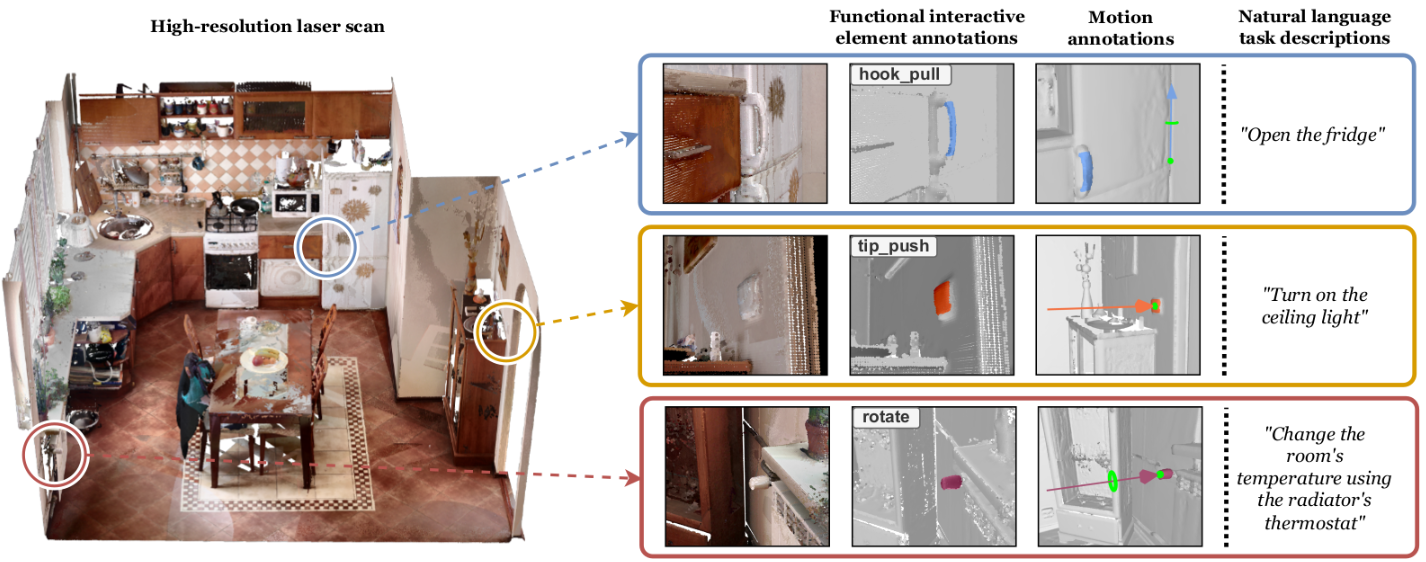
\includegraphics[width=\textwidth]{content/images/SceneFun3D.png}
    \caption{SceneFun3D tasks visualised \cite{delitzas2024scenefun3d}}
    \label{fig:your_image_label}
\end{figure}
\cref{fig:your_image_label} shows the expected output of all the three tasks. Functionality segmentation refers to segmenting out the functional interactive 
element from the given scene and annotating it with one of the eight affordance labels defined by \cite{gibson}. Task-driven affordance grounding refers to the task
of associating a text query in the context of the scene to the functional element that can be manipulated for the given text description. Finally, motion estimation
aims to provide the motion parameters that the agent should perform in order to successfully interact with the functional element.

Further, SceneFun3D also provides a well-defined dataset of 720 recorded scene from the ARKITscenes dataset and various assets for each scene 
to train deep learning models that can tackle these problems. They provide the following assets, RGB-D images, poses, accurate laser scans, 
annotations for each element present in the dataset, motion parameters for each annotation and task description in natural language for every function element.
In our thesis, we aim to beat the baseline results obtained by \citet{delitzas2024scenefun3d} for the first two tasks, namely 
functionality segmentation and task-driven affordance grounding. 

\subsection{3D scene graphs:}
The term scene graph was first introduced in \cite{7298990}, as a novel framework for retrieval of images. Here, the authors designed the scene graph which 
consists of three sub-parts, the nodes, the edges and the attributes for each node. First, let us understand the definition of a scene graph and later
look at its evolution to 3D. 
A scene graph can be defined as a structural representation of a particular scene which captures semantically rich information about the objects in that scene \cite{zhu2022scenegraphgenerationcomprehensive}.
This is done by explicitly modelling the objects, their attributes and the relationship between paired objects as seen in \cref{fig:2dvs3dSG}. The objects appear to be in boxes as nodes
and the spatial relationships are given by edges connecting the nodes.
In short, it is called a “scene graph” because it organizes all this information as a graph: the objects are represented as nodes with their attributes, and the edges between these 
nodes are the relationship between these objects. 

For a robot to navigate around its environment and interact with the objects in its vicinity, it first needs to have a semantically rich map of its surroundings. 
This surrounding area where the robot can move and interact is called the scene and the semantically rich map must contain the 
semantic data of all the objects in the scene as well as their locations and inter-object relationships. 
A 3D scene graph can be used to store this kind of semantically rich data of the objects of the robot’s surroundings. 

A 3D scene graph is an extension of the traditional scene graph. It is a spatial representation of the objects, their attributes 
and their relationships in three dimensions, in short, they store 3D information. The objects in 3D scene graphs are modelled as
 3D point clouds and they visually resemble the original object. The distinction between a normal scene graph and a 3d scene graph 
 can be seen from the \cref{fig:2dvs3dSG}
 \begin{figure}[ht!]
    \centering
    \includegraphics[width=\textwidth]{content/images/2dvs3dSG.png}
    \caption{3D (bottom left) vs 2D (bottom right) scene graph for given scene of two arm chairs (top)}
    \label{fig:2dvs3dSG}
\end{figure}
To further elaborate on 3D scene graphs, consider the example of a scene where an armchair is next to another armchair.
The scene graph here consists of two nodes;
the first node is the armchair with “red" as an attribute, and the second node is the second armchair with "red" as an attribute. The spatial relation, 
"next to” is given an edge. Thus, the scene graph provides a compact representation of the scene to the robot. 
An example can be seen from our implementation in the \cref{fig:2dvs3dSG}.

\subsubsection{Uses of 3D Scene Graph}
As we discussed above the scene graph can be leveraged by a robot to navigate around a scene and complete its tasks by manipulating objects defined in the task. 
Apart from this, there are numerous other tasks which can be accomplished using either a traditional scene graph or a 3D version of it. Scene graphs have been 
used to enhance image generation \cite{tripathi2019usingscenegraphcontext}, \cite{johnson2018imagegenerationscenegraphs}, 
the relationships between the nodes are leveraged to incorporate meaningful information during the image generation process to get realistic images.
 Other uses include image captioning using scene graphs \cite{8953305}. 
 Scene graphs can also be used to detect visual relationships between objects in an image, Visual question answering, semantic image retrieval and many more. \\
Before moving to the generation of 3D scene graphs, we will look at the tools used during this process. 
These tools are mainly machine learning and deep learning models. Scene graphs are generated from RGB-D images and poses. 
Out of these, RGB images play an important role in providing semantic information to the scene graph. RGB images are used for object detection,
object segmentation, relationship building and caption generation. All of these tasks are possible due to one or more AI models.
Mainly foundation models like Visual Language Models such as LLaVA and Chat Gpt 4 are used for caption generation and 
relationship building, and SAM for object segmentation. Along with this, object detection models like YoLo form the basis of 
3D scene graph generation. 
Next, let us look at the theoretical concepts behind these models and then have a look at how they help in scene graph generation.
\subsection{Foundation models:}
Foundation models can be defined as large-scale, pre-trained models that can perform various downstream tasks\cite{bommasani2022opportunitiesrisksfoundationmodels}. 
Foundation models have two reasons for being successful, scale and transfer learning. On one hand, Scale represents,
more computing power in terms of CPU, GPU and memory and a large amount of multimodal training data. Such data is gathered from 
massive datasets generated across diverse domains, this makes generalization possible in foundation models. On the other hand, transfer
learning takes the learnings from one task (e.g., object recognition in images) and
applies them to another task (e.g., activity recognition in videos). 
\begin{figure}[ht!]
    \centering
    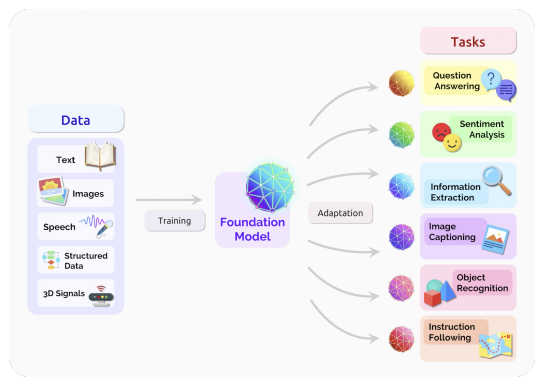
\includegraphics[width=\textwidth]{images/FoundationModels.png}
    \caption{Foundation model overview.}
    \label{fig:foundation_model}
\end{figure}
From \cref{fig:foundation_model} we can see that, 
a foundation model gathers the knowledge from all the data from various data sources such as texts, images, videos and many more.
This model then adapts to a wide range of downstream tasks such as question answering, sentiment analysis, and object detection just to 
name a few. Their applications range from natural language processing (NLP), and computer vision (CV) to robotics and more. 
Let us look at some of the foundation models we will be using in our scene graph implementation.

\subsubsection{Segment Anything model [https://arxiv.org/abs/2304.02643]:}
The paper by \citet{kirillov2023segment} first introduced the Segment Anything Model (SAM). SAM is developed by Meta FAIR. 
This foundation model can segment any given 2D image. Segmentation can be made using the following ways, 
it can be prompted with interactive points and boxes, it can automatically segment everything in the image without a prompt, 
and generate multiple masks for ambiguous prompts. According to Meta AI, “Sam has learned a general notion of what objects are – this understanding enables zero-shot generalization to 
unfamiliar objects and images without requiring additional training.”. The outstanding accomplishments of SAM are possible due to the fact that
the authors used a large number of masks approximately 1 billion masks from 11 million images to train the model. Due to such a large dataset, 
the model has learnt to segment almost anything out of a given image, hence the name Segment Anything Model. In the figure below we can see the segmentation results from SAM.
A glimpse of SAM can be seen in the \cref{fig:sam}
\begin{figure}[ht!]
    \centering
    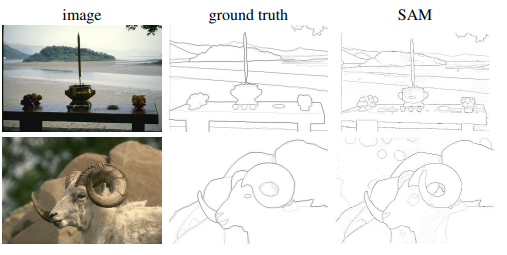
\includegraphics[width=\textwidth]{content/images/SAM.png}
    \caption{Foundation model overview. \cite{kirillov2023segment}}
    \label{fig:sam}
\end{figure}
\subsubsection{Vision Language Models (VLMs):}
VLMs are advanced machine learning models able to process visual and textual data. VLMs are also foundation models as they are trained on multimodal data such as text, images,
videos and many more. Moreover, the ability of VLMs to generalize and provide answers to any given task may it be question answering, object detection or sentiment analysis makes
them worthy of foundation models. They can generate outputs based on their understanding of the multimodal input provided to them. 
In this chapter, we will be looking at the two most used VLMs, ChatGPT-4 and LLaVA.

\textit{ChatGPT-4:}
The onset of the Large Language Model (LLM) in today's world has opened many possibilities for the use of AI. One such use is chatbot applications or AI
assistants. ChatGPT is a foundation model developed by OpenAI. ChatGPT was made public in November 2022. Initially, ChatGPT was only capable of 
text-based queries but performed well in question-answering tasks. It showed human-like rationale. However, it had limitations such as 
only a single mode of input and output (text) and it was poor in mathematical reasoning. Since then ChatGPT has evolved and today the successor 
Chat-GPT4 has not only overcome previous limitations but also improved logical and rational reasoning. ChatGPT-4 showed more than 20\% increase in overall accuracy
on the  United States Medical Licensing Examination (USMLE) sample test and AMBOSS questions \url{https://www.amboss.com/us}. Moreover, ChatGPT-4 
also has multimodal input and output capabilities, making it suitable for visual question-ansewering. Visual question-answering is the task where
the model is given an image or a video and is asked questions related to the data provided. The questions are for example, 'Describe the scene given in 
the image.', 'What color is the table in the given image' or 'Is there a chair present in the scene? What is its spatial relationship with the table?'

\textit{Large Language and Vision Assistant:}
 Large Language and Vision Assistant (LLaVA) is an end-to-end large multimodal model trained on data generated with the help of GPT-4 \cite{liu2023visualinstructiontuning}. 
 It connects the vision encoder and LLM for general-purpose visual and language queries. LLaVA performs well on vision queries. 
 Vision queries are queries where the model is provided with an image and a general query is asked regarding the image. 
 For eg, An image with a room is provided and the query can be, ”Is there a computer present in this image?”. LLaVA is an open-source model which is available on
 hugging face. It is a cost-effective alternative to ChatGPT with great performance but not at par with ChatGPT. LLaVA provides an API format with which queries can be made
 to the model by downloading it locally. The API expects an image and a prompt in the query. In the code snippet given below, we instantiate the model and its processor. We
 query LLaVA using an image of a water bottle on a table and ask the following query, \enquote{Please describe the given image.} \cref{fig:llava} shows the image
 and the output.  
\begin{lstlisting}
from transformers import LlavaNextProcessor, LlavaNextForConditionalGeneration, BitsAndBytesConfig
import torch
from PIL import Image

processor = LlavaNextProcessor.from_pretrained(model_id)
bnb_config = BitsAndBytesConfig(
                            load_in_4bit=True, bnb_4bit_use_double_quant=True,
                            bnb_4bit_quant_type="nf4", bnb_4bit_compute_dtype=torch.bfloat16)
model = LlavaNextForConditionalGeneration.from_pretrained("llava-hf/llava-v1.6-vicuna-13b-hf", 
                                                          torch_dtype=torch.float16, 
                                                          low_cpu_mem_usage=True, 
                                                          quantization_config=bnb_config,
                                                          use_flash_attention_2=True ) 
torch.set_default_dtype(torch.float16)
image = Image.open("sceneGraph3D/conceptgraph/scripts/frame000090annotated_for_vlm.jpg")
conversation = [
    {
      "role": "user",
      "content": [
          {"type": "text", "text": "Please describe the given image."},
          {"type": "image"}
        ],
    },
]
prompt = processor.apply_chat_template(conversation, add_generation_prompt=True)
inputs = processor(images=image, text=prompt, return_tensors="pt")
output = model.generate(**inputs, max_new_tokens=500, do_sample=False)
print(processor.decode(output[0], skip_special_tokens=True))
\end{lstlisting}

\begin{figure}[ht!]
    \centering
    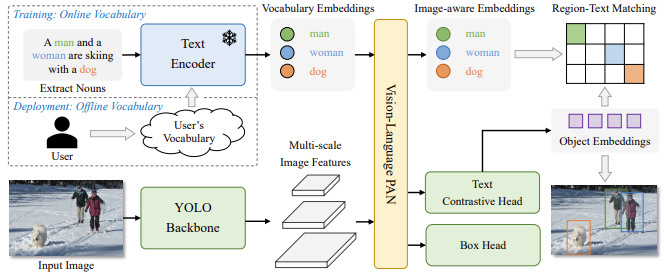
\includegraphics[width=\textwidth]{content/images/YOLOWorld.png}
    \caption{High-level working of YOLO-World \cite{cheng2024yolow}}
    \label{fig:llava}
\end{figure}
 LLaVA can perform more complex tasks such as scene understanding or identifying spatial relationships, the example for this is given in \cref{chap:k7}.

\subsection{Object segmentation:}
The task of separating an object from its background and other surrounding objects is called object segmentation. Object segmentation divides an image or 3D point cloud
 into meaningful regions, it labels each pixel or point to delineate the boundaries of different objects in the given scene. There are traditional methods like edge detection, 
 thresholding, and region growing which can segment out images. However, these methods do not provide good results in terms of semantic segmentation, where the segments must 
 have semantic information as a whole. For example, segmenting out a chair from a room. This is because traditional methods purely rely on 
 pixel-level features such as intensity, gradients, or texture, without understanding the context of objects present in the scene. However, newer methods like convolutional
 neural networks such as Mask R-CNN, transformer-based methods like SAM and point cloud networks like PointNet ++ are capable of semantic segmentation. 
 There are two types of object segmentation:
 \begin{compactenum}[1.]
    \item	Semantic segmentation.
    \item	Instance segmentation.
 \end{compactenum}
\begin{figure}[ht!]
    \centering
    \includegraphics[width=\textwidth]{content/images/segmentation_sem_vs_inst.png}
    \caption{Input image (top left), Semantic segmentation (top right), Instance segmentation (bottom right), Object detection (bottom left)}
    \label{fig:segmentation_sem_vs_inst}
\end{figure}
The difference between the two is that the former segments out object classes but doesn't consider objects under the same class as distinct segments whereas, the instance segment 
considers each segment as unique and identifies the obejcts in each class and consider them as a separate instances within the class. The difference can be understood by looking at 
\cref{fig:segmentation_sem_vs_inst} \cite{Sharma2022}. If we look at the top right part of the figure we see that there are two distinct colors yellow and red representing two
classes, nuts and bolts. Whereas, in the bottom right corner we can see each instance of the class nut has different colours and the same can be said for the class bolt.
\subsection{Open-vocabulary obejct detection:}
The task of identifying an object and locating its position in an image is called object detection. Until recently, object detection was limited to a small and fixed
set of classes. This limitation was due to the fact that obtaining a large training dataset with diverse classes is time-consuming and costly. \cite{10.1007/978-3-031-20080-9_42} 
The limitations of traditional object detection can be overcome using open-vocabulary object detection, a method where the model can detect the class of an 
object beyond its training set. Open-vocabulary object detection is a powerful method enabled by the advancements in powerful language encoders 
and contrastive image text training models like CLIP. 

One such model is YOLO-World by \citet{cheng2024yolow}, an approach to enhancing open vocabulary object detection capabilities in You Only Look Once (YOLO).
YOLO is a series of object detection models which are light-weight and effective. 
\begin{figure}[ht!]
    \centering
    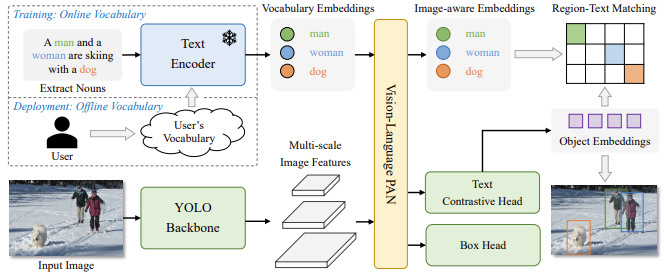
\includegraphics[width=\textwidth]{content/images/YOLOWorld.png}
    \caption{High-level working of YOLO-World \cite{cheng2024yolow}}
    \label{fig:yolo}
\end{figure}

The architecture of YOLO-World is given in \cref{fig:yolo}, it consists of a YOLOv8 detector, a Text encoder, and a Re-parameterizable Vision-Language
Path Aggregation Network (RepVL-PAN) \cite{cheng2024yolow}. Along with image the YOLO-World model also adopts text as input. The Text encoder is adopted
from a CLIP pretrained Transformer text encoder and it encodes the input text into text embeddings. The image is transformed into multi-scale image features using the 
YOLO backbone. The RepVL-PAN then enhances both text and image representation by fusing the image features and text embeddings. Finally, bounding boxes and object 
embeddings for matching the classes that appear in the input are predicted.

Applications for open-vocabulary object detection (OOVD) range from robotics to healthcare. In robotics, scene understanding, warehouse automation and household
assistance can be enhanced, the robots can predict unseen objects and understand the scene semantically better thus enabling human-like behaviour. In fields like Autonomous 
driving and security, OOVD can assist in detecting anomalies where the traditional object detection models may fail. The anomalies can be pedestrians, debris and
 road signs in autonomous driving or unattended baggage and unfamiliar objects in security surveillance.

 Despite its impressive capabilities, OOVD has many limitations that hold back its widespread adoption and accuracy in the real world. Some of the key limitations 
 include:
 \begin{compactenum}[1.]
    \item Generalization and accuracy: OOVd models struggle with rare categories for objects that lack visual-textual data in the training of text encoders like
    CLIP. Lack of expertise in domain-specific applications, as the OOVD models are good at generalization. 
    \item OOVD models depend on textual descriptions, limiting their performance to the quality of the text encoders used. Another limitation is the 
     language barrier as most text encoders are tarined in the English language, thus limiting the OOVD to English text descriptions. 
 \end{compactenum}
\subsection{Generating scene graphs using foundation models:}

\let\cleardoublepage\clearpage
\chapter{Methodology}
\label{chap:k4}
In the chapter, we will look at the methodology used to realise the milestones set in \cref{chap:k1}. We first list the approach
followed during the realisation of this thesis. Next, we propose a solution for the limitations we saw in \cref{chap:k2} and then
we give a detailed description of the system design and its main components. Finally, we deep dive into the implementation details.

% \section{Research Approach:}
% \begin{compactenum}[1.]
%     \item Implement the state-of-the-art scene graph generation framework, ConceptGraphs.
%     \item Gather dataset by recording scenes manually in the SIR lab.
%     \item Verify the implementation using pre-recorded, synthetic and captured datasets.
%     \item Extend the implementation by including a novel way to segment part from an object in the existing ConceptGraphs
%     \item Test multiple methods to segment part from an object
%     \item Evalute methods and feasibility
%     \item Integrate the method into current implementation
%     \item Test and Validate the new implementation after integration
%     \item Present Results using Average Precision metrics and Snapshots of the output


\section{Approach}
The study utilizes a systematic approach to create, enhance, and evaluate a framework for scene graph generation. The subsequent are the essential steps:
\begin{compactenum}[1.]
\item \textbf{Implement the ConceptGraphs:} Utilize ConceptGraphs, a state-of-the-art framework for scene graph generation.
\item \textbf{Dataset Collection:} Capture a real-world dataset by recording real-world scenes within the SIR laboratory.
\item \textbf{Execution:} To ensure accuracy and correctness, verify the implementation with pre-recorded and synthetic datasets.
\item \textbf{Part-Object segmentation:} Develop and test an innovative method for segmenting part and object within the ConceptGraphs framework.
\item \textbf{Incorporating ConceptGraphs:} Integrate the segmentation method into the existing ConceptGraphs implementation.
\item \textbf{Verification of Part-Object Segmentation:} To guarantee the enhanced implementation's accuracy and reliability, do comprehensive testing.
\item \textbf{Evaluation and Examination: } Assess several segmentation methodologies based on their average precision and feasibility.
\item \textbf{Results: } Use Average Precision (AP) metrics to evaluate the completed system, and illustrate  qualitative results with the help of output snapshots.
\end{compactenum}
\let\cleardoublepage\clearpage
\section{Proposed solution}
\label{chap:k5}
We saw the limitations current scene graph generation methods possess in terms of functionality segmentation of interactive elements. We also
saw the importance of having such a fine-grained understanding of a scene at the interactive element level. Therefore, we propose a novel way of
extending the current implementation of \cite{gu2023conceptgraphsopenvocabulary3dscene} by adding functionality segmentation as a part of its process while generating the 
scene graph. For this, we plan on training point cloud neural networks as well as transformers on a dataset which has annotations for both the
object and its part. Such a dataset is one of its kind and will be formed by merging two datasets, SceneFun3d and ARKit LabelMaker.
The SceneFun3D dataset has annotations for various functional interactive elements and categorises them into eight classes namely,
tip\_push, hook\_turn, hook\_pull, pinch\_pull, key\_press, unplug, plug\_in and rotate. The ARKit LabelMaker dataset derives itself from ARKITscenes dataset
by Apple, they build an automatic pipeline to segment out objects from the ARKITscenes point clouds by first segmenting the objects in 2D and 
then lifting these segments to 3D. As both these datasets are in the same co-ordinate world we plan to merge them and carve out part-object
point clouds for training the neural networks and transformers. Later, we propose another innovative idea of using the scene graph for 
task-driven affordance grounding. For this, the scene graph will be given a language-based task description and it will be expected to return
task-driven affordance grounding. For this, the scene graph will be given a language-based task description and it will be expected to return
the interactive segment that can be used to complete the task. Generally, each functional interactive element is associated with an object.
We plan to retrieve this object by using the scene graph and later pass this object to the pre-trained neural network and Transformer to get
segmentation. In this segmentation we expect the object segmented out from its part, which will be the answer to the task description given in 
segmentation. In this segmentation we expect the object segmented out from its part, which will be the answer to the task description given in 
natural language.
\let\cleardoublepage\clearpage
\section{Design}
\label{chap:k6}
In this section, we will look at the high-level design of our implementation. We will define the individual components in our
implementation and show how they are connected and how data flows between them.

\subsection{Design}
Our implementation has three important parts, data pre-processor, scene graph generator and query handler. The query handler will also visualise
the answers to the query. In the \cref{fig:system_desgin} you can see the pictorial representation of the three parts as boxes and the connections depict the data flow.
\begin{figure}[ht!]
    \centering
    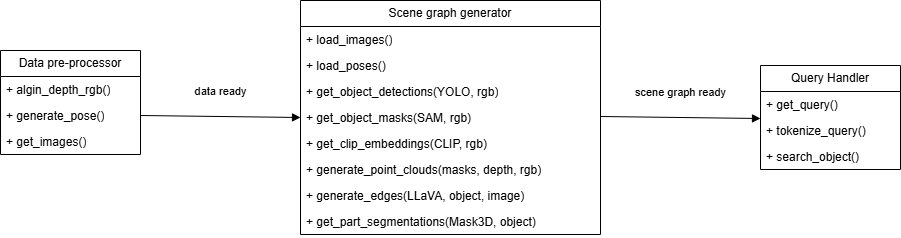
\includegraphics[width=\textwidth]{content/images/Design.png}
    \caption{System design}
    \label{fig:system_desgin}
\end{figure}

We will dive deep into the details of each component one by one. First, we will look at the data pre-processor, next the scene graph generator and finally 
the query handler.

\subsubsection{Data pre-processor}
The data pre-processor is responsible for transforming the raw data from various sources into the format expected by ConceptGraphs. 
ConceptGraphs expects a sequence of RGB-D images and camera poses. Therefore, we need a data pre-processor that can handle various formats of data
and parse them into the expected one.  We mainly focus on data from robots and the cameras mounted on the robots, due to the fact that our system's end goal 
is to assist the robot in task fulfilment. 
Therefore, we will focus on rosbag and .mkv files for RGB-D image sequences. The reason for considering these two data formats is that during our experiments
we will have access to only rosbags and .mkv files obtained from Intel Realsense camera and Femto Bolt by ORBBEC respectively. Moreover, .rosbag is a widely used format in robotics.
The data pre-processor will parse the rosbags and .mkv files  and get a sequence of aligned RGB-D images. 
The RGB and D images must be aligned. The reason for requiring alignment is, that the scene graph 
generator will detect objects from RGB images and from the corresponding depth images it will generate the point clouds and assign colours from 
the RGB images. Thus, alignment is necessary for avoiding wrong colours and malformed objects. \cref{chap:k7} provides the detailed 
implementation point cloud generation. 
Further, the data pre-processor will also be responsible for loading the camera poses. The camera poses can either be absent or be in 
a different format. In the first case, we will use SfM software for obtaining poses from RGB images. In the second case, we will need to
ensure that all the poses are transformed into camera-to-world coordinates which is expected by concept graphs.
\begin{figure}[ht!]
    \centering
    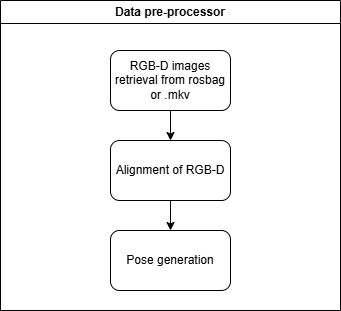
\includegraphics[width=0.5\textwidth]{content/images/DataPreProcessorDesign.png}
    \caption{Internal components of data pre-processor}
    \label{fig:dataPreprocessor}
\end{figure}
In the \cref{fig:dataPreprocessor}, we can see the sub-components of the data preprocessor.

\subsubsection{Scene graph generator}
The scene graph generation is the central component in our system that handles computationally heavy workloads. Therefore, it makes sense to have an 
in-depth look at this particular component. The scene graph generator is responsible for taking RGB-D image sequences and poses as an input and giving queryable scene graphs
as an output. The final scene graph must be able to handle text queries and return a functional interactive element or an object as an answer to the query. \\
\begin{figure}[ht!]
    \centering
    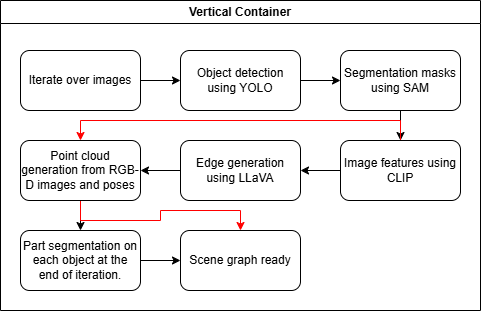
\includegraphics[width=0.5\textwidth]{content/images/SceneGraphGenerator.png}
    \caption{Internal components of scene graph generator}
    \label{fig:sceneGrahpGenerator}
\end{figure}
To generate a scene graph from a set of images we will take the aid of four machine learning models, LLaVA, SAM, YOLO and CLIP. First, we will use YOLO to detect 
objects from given RGB images, YOLO provides bounding boxes and class labels for each detected object. Later, we will employ SAM to get the mask for these detected 
objects, by passing the image and the bounding box to SAM, it will segment out the exact mask for the desired object. We will pass the same image to CLIP
in order to get textual embedding for the image, these embeddings will be used later while querying to find similarities between objects and the query. 
Each object generated from this pipeline will be passed to a VLM like LLaVA to get spatial relationships (edges) between the objects detected. Finally,
we will generate the point cloud for each object using the masks from SAM, the depth values from D images and camera poses for each image. This point cloud
will be passed to a neural network or a transformer to perform part segmentation and segment out functional interactive elements. This way a scene graph will be generated where objects will be
the nodes for this graph and the spatial relationships will be the edges. The scene graph will be then passed to the next component for handling queries.
The tasks of edge generation and part segmentation can be skipped to enable faster scene graph generation, 
this is depicted by red lines in the \cref{fig:sceneGrahpGenerator}.
\subsubsection{Query handler}
This is the last component in our system as depicted in \cref{fig:queryHandler}. It will take a textual query as an input and return a functional element or an object as an answer to the query. The central
part of this component is the CLIP model which will tokenize the input query and then find the most similar objects from the scene graph. The similarities are found 
by finding the cosine similarities between the input query and all the text embeddings generated for each object in the scene graph in the last component using CLIP.
The object with the most similarity is returned as the most probable output, with the remaining objects given weights according to the probabilities. A heat map is 
generated using these probabilities and displayed as a scene graph.\\
\begin{figure}[ht!]
    \centering
    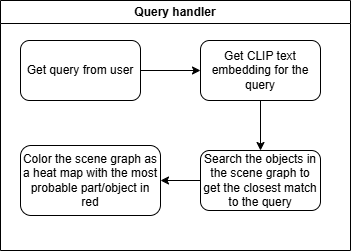
\includegraphics[width=0.5\textwidth]{content/images/QueryHandler.png}
    \caption{Internal components of query handler}
    \label{fig:queryHandler}
\end{figure}

In conclusion, this was the overall design of our proposed system. These are three main components namely, data pre-processor, scene graph generator and query handler. 
The data flow between the components is given in the figure and is linear. Next, we will look at the plan to implement this design, test it and get results.

\let\cleardoublepage\clearpage
\section{Implementation}
\label{chap:k7}
In this section, we will begin with the actual implementation of the proposed solution. The implementation section will list the challenges faced and
the tasks completed during the thesis. It also provides unique solutions to each of them. This will provide necessary details into the methods used and will
enable a better understanding of the overall implementation process. Along with this, we will list the hardware and software components 
used in our system and provide the steps and code for the important components in our system. 
The hardware and software specifications are documented to ensure reproducibility and provide
insights into the computational costs required for similar research in the future. The pseudo-code and algorithms are not the actual code implemented
during the thesis but just an abstraction of the original idea. The software libraries evolve, thus, we plan to maintain the code for
future versions in the following GitHub link: \url{https://github.com/ChinmayNadgouda/sceneGraph3D/tree/concept-graph}.

\subsection{Software Specifications}
The software environment and tools utilized are summarized in Table \ref{tab:software_specs}. These requirements are strict as there are inter-dependencies
between many Python libraries. For later versions of the following libraries, necessary changes need to be made as per the updates in that specific library.

\begin{table}[ht]
    \centering
    \caption{Software Specifications}
    \label{tab:software_specs}
    \begin{tabular}{lll}
        \toprule
        \textbf{Software}      & \textbf{Version}   & \textbf{Purpose}                     \\
        \midrule
        Python                & 3.10               & Core development                      \\
        PyTorch               & 2.1                & Deep learning framework               \\
        Open3D                & 0.17               & Point cloud processing                \\
        COLMAP                & 3.9                & 3D reconstruction                     \\
        CUDA                  & 11.8               & GPU acceleration                      \\
        Anaconda              & 2023.07            & Environment management                \\
        Git                   & 2.42               & Version control                       \\
        \bottomrule
    \end{tabular}
\end{table}
\subsection{Hardware Specifications}
The hardware setup used for the experiments is detailed in \ref{tab:hardware_specs}. It includes the Specifications of the system
used to develop and test the proposed solution. Although these specifications are not strict requirements, we found these to work best for our
thesis.

\begin{table}[ht]
    \centering
    \caption{Hardware Specifications}
    \label{tab:hardware_specs}
    \begin{tabular}{ll}
        \toprule
        \textbf{Component}      & \textbf{Specification}              \\
        \midrule
        CPU                     & Intel Core i7-12700H, 14 cores, 4.7 GHz \\
        GPU                     & NVIDIA RTX 3090, 24GB GDDR6X          \\
        RAM                     & 32GB DDR5                             \\
        Storage                 & 1TB NVMe SSD                          \\
        Operating System        & Ubuntu 22.04 LTS (64-bit)             \\
        \bottomrule
    \end{tabular}
\end{table}



Listed in \cref{tab:software_specs} and \cref{tab:hardware_specs} are the specifications and requirements of our system. Now, we will look at the implementation details of the finer concepts in the 
three components we saw in \cref{chap:k6}.

We will dive step by step into the main implementation concepts, Pose generation, Image extraction and alginment, ConceptGraphs implementation, 
training Mask3D and PointNet++, integration of Mask3D and PointNet++ with Concept Graph, and Query handling.

\subsection{Pose generation}
The Intel Realsense Depth Camera D435 \cite{camera} was used for recording the scene at our lab. 
While we recorded the scene, we faced the challenge of determining poses for the recorded camera images from our Realsense camera. The realsense camera provides IMU extrinsic
values but they are not useful in our case. For the purpose of 3D reconstruction from a sequence of RGB-D images, it is essential to have ground truth camera poses. This 
can be achieved either by using external setups like, Global Positioning System (GPS) or software like COLMAP can be utilised. In our thesis, we focus on using COLMAP,
which is a structure from motion software. 

COLMAP takes the sequence of RGB images as an input and gives the ground truth pose in the world to camera (w2c) coordinates. However, ConceptGraphs expects camera to world (c2w)
coordinates and the world axes of the two are not aligned. Therefore we had to apply the transformation matrix given in \cref{lst:pose}. The COLMAP outputs are w2c poses and can be found 
in images.bin or images.txt files. The poses are given line by line and each line has nine entries. The first four entries are quaternions, the next 3 are translations and the remaining entries are
not useful for pose estimation. The sample code snippet is given in \cref{lst:pose}.

We refer the transformation steps given in \cite{colmap2nerf} by \citet{mueller2022instant}. 

\subsection{Image extraction and Alginment}
Intel provides a ROS wrapper for the Realsense D435  camera. Therefore the output is a rosbag for the recorded video. This rosbag consists of sequential RGB-D images for each time
stamp. The image resolution for RGB images is 1920~$\times$~1080p and the image resolution for depth images is 1280~$\times$~720p. As a result, the pixels from colour images are not aligned with the depth pixels due to 
resolution mismatch, different fields of view (FoV) and physical separation of depth and colour cameras. Therefore, we leverage the Python package pyrealsense2 provided by Intel to align the depth and colur images. 
The brief code for the following is given in \cref{lst:align} and algorithm in \cref{alg:process_rosbag}.
\begin{Algorithmus}
  \caption{Processing ROSBag File Using RealSense SDK}
  \label{alg:process_rosbag}
  \begin{algorithmic}[1]
    \Require $\mathsf{fname}$ \Comment{\texttt{Path to the .rosbag file}}
    \State $\mathsf{pipeline} \gets \mathsf{load\_config\_and\_rosbag(fname)}$ \Comment{\texttt{Load ROSBag file}}
    \State $\mathsf{align\_to} \gets \mathsf{get\_alginment\_method(color)}$
    \While{True}
      \State $\mathsf{frames} \gets \mathsf{pipeline.wait\_for\_frames()}$   \Comment{\texttt{Iterate over frames}}
      \State $\mathsf{aligned\_frames} \gets \mathsf{align.process(frames)}$  \Comment{\texttt{Align Frames}}
      \State $\mathsf{aligned\_depth\_frame} \gets \mathsf{aligned\_frames.get\_depth\_frame()}$ 
      \State $\mathsf{color\_frame} \gets \mathsf{aligned\_frames.get\_color\_frame()}$
      \If { !$\mathsf{aligned\_depth\_frame}$ or !$\mathsf{color\_frame}$}  
        \State \textbf{continue}                            \Comment{\texttt{Skip if no frame found}}
      \EndIf
      \State $\mathsf{depth\_image} \gets \mathsf{algined\_depth\_frame}$
      \State $\mathsf{color\_image} \gets \mathsf{color\_frame}$
    \EndWhile
    \State $\mathsf{pipeline.stop()}$
  \end{algorithmic}
\end{Algorithmus}

The RGB images are used for object detection as well as segmentation using SAM whereas the depth images provide distance values of each pixel.
The SAM masks and the depth values play an important role in forming the point clouds. To avoid distorted point clouds in the final scene graph 
alignment of the RGB-D images is paramount.

\subsection{ConceptGraphs implementation}
In our thesis, we have utilised a state-of-the-art method for generating scene graphs, ConceptGraphs \cite{gu2023conceptgraphsopenvocabulary3dscene}.
 The implementation for ConceptGraphs is already present on GitHub. We will dive deep into the implementation details of this open-source method developed by \citet{gu2023conceptgraphsopenvocabulary3dscene}.

First, we will have a look at the configuration files and the overall requirements of this method. Later, we will introduce the models and steps taken one by one, starting 
with YOLO for object detection, SAM for segmenting the detected objects and obtaining masks for the objects. Next, we will look at the detailed implementation to 
obtain spatial relationships and image-object captions using VLMs like CLIP and LLaVA. All these steps are iterated over all the images for the provided dataset. After each iteration, 
the detected objects are stored and logged into a rerun viewer for visualisation. These newly detected objects are compared visually and semantically with the 
objects stored in the previous iteration. Objects which are similar to existing objects are merged. Finally, we will look at the novel extension proposed by this thesis. 
We propose the addition of the trained models like Mask3D and PointNet++ in the last iteration. In the last iteration, we will have all the objects detected so far. We will
loop over these objects and their point clouds will be passed to Mask3D or PointNet++. The model will then segment out the parts for the given objects. The parts obtained from
the models will be given a label and five textual descriptions, these textual descriptions for each part will be related to the tasks that can be performed by it as a composition
of its parent object. The objects are stored in a detection list with the following schema. 
\begin{lstlisting}
  detected_object = {
  'id' : uuid.uuid4(), 
  'image_idx' : [image_idx],     # idx of the image
  
  'mask_idx' : [mask_idx],       # idx of the mask/detection
  'color_path' : [color_path],   # path to the RGB image
  'class_name' : curr_class_name,   # global class name for this detection
  'class_id' : [curr_class_idx],    # global class id for this detection
  'captions' : [gobs['captions'][mask_idx]],  # captions for this detection
  'num_detections' : 1,            # number of detections in this object
  'mask': [gobs['mask'][mask_idx]],   #from yolo
  'xyxy': [gobs['xyxy'][mask_idx]],    #from yolo
  'conf': [gobs['confidence'][mask_idx]],    #from yolo
  'n_points': len(obj_pcds_and_bboxes[mask_idx]['pcd'].points),                       
  "inst_color": np.random.rand(3),  # A random color used for this segment instance
  'is_background': is_bg_object,    # background classes are wall, floor and roof
  
  # These are for the entire 3D object
  'pcd': obj_pcds_and_bboxes[mask_idx]['pcd'],   #from point cloud
  'bbox': obj_pcds_and_bboxes[mask_idx]['bbox'],  #from point cloud
  'clip_ft': to_tensor(gobs['image_feats'][mask_idx]),  #from CLIP
  'num_obj_in_class': num_obj_in_class,
  'curr_obj_num': tracker.total_object_count,
  'new_counter' : tracker.brand_new_counter,
}
\end{lstlisting}

The fields xyxy and conf will be obtained from YOLO. The field mask will be obtained from SAM.
The fields pcd, bbox and n\_points will be obtained from the point cloud generation algorithm. The field clip\_ft is the 
CLIP embedding from CLIP and captions will be generated by LLaVA. We will see the implementation pseudo code for each below.

\subsubsection{YOLO object detection}
ConceptGraphs utilise the YOLO-Worl model, which shows great performance for open vocabulary object detections. At every iteration, YOLO detects the objects in the image
 from a given list of classes. These classes can be given runtime or can be inferred from CLIP. YOLO returns the class\_id of the detected object which corresponds to the index of the class list provided.
 It also returns the bounding boxes and confidences for each object. 
 \begin{Algorithmus}
  \caption{Object Detection using YOLO}
  \label{alg:get_object_detections}
  \begin{algorithmic}
    \Procedure{get\_object\_detections}{$YOLO, rgb$}
      \State $\mathsf{detection\_model} \gets YOLO('yolov8l-world.pt')$
      \State $\mathsf{image} \gets \mathsf{load(\textit{rgb})}$ \Comment{\texttt{Read RGB image}}
      
      \State $\mathsf{results} \gets \mathsf{detection\_model.predict(image, conf=0.1)}$    \Comment{\texttt{predict}}
      \State $\mathsf{conf} \gets \mathsf{results.boxes.conf}$    \Comment{\texttt{Get confidence score}}
      \State $\mathsf{detection\_class\_labels} \gets \mathsf{results.labels}$  \Comment{\texttt{Get class label}}
      \State $\mathsf{xyxy} \gets \mathsf{results.boxes.xyxy}$   \Comment{\texttt{Get bounding box}}
      
      \State \Return $\mathsf{conf, detection\_class\_labels, xyxy}$
    \EndProcedure
  \end{algorithmic}
\end{Algorithmus}


\subsubsection{SAM segmentation}
In the next step, we will pass the same image along with the bounding boxes to SAM. This will be the prompt for SAM, the bounding boxes dictate
 the area where SAM must perform segmentation and return the corresponding masks.
 \begin{Algorithmus}
  \caption{Get Object Masks using SAM}
  \label{alg:get_object_masks}
  \begin{algorithmic}
    \Require $\mathsf{\textit{SAM, rgb, b\_box}}$
    \Ensure $\mathsf{mask}$

    \State $\mathsf{sam\_predictor} \gets \mathsf{\textit{SAM}('mobile\_sam.pt')}$ 
    \Comment{\texttt{Initialize UltraLytics SAM model}}

    \If {$\mathsf{exists(\textit{b\_box})} $} 
        \Comment{\texttt{Check if bounding boxes exist}}
        \State $\mathsf{sam\_out} \gets \mathsf{sam\_predictor.predict(\textit{rgb, b\_box})}$
        \Comment{\texttt{Run segmentation model}}
        \State $\mathsf{mask} \gets \mathsf{sam\_out.masks.data}$
    \Else
        \State $\mathsf{mask} \gets \mathsf{None}$
        \Comment{\texttt{Return empty mask if no bounding box is found}}
    \EndIf

    \State \Return $\mathsf{mask}$
    
  \end{algorithmic}
\end{Algorithmus}

\subsubsection{CLIP embeddings}
CLIP will be used to obtain the image features in text form which are embedded using CLIP itself. The embeddings are for individual objects and hence we crop 
out the object from the original image using the bounding boxes earlier provided by YOLO. We process all the cropped images in batches, the class for each object is 
also encoded and fed to the CLIP model. This ensures better performance in obtaining accurate feature embeddings. The feature embeddings represent the image in a 
high-dimensional space, capturing semantic similarities.
\begin{Algorithmus}
  \caption{Extract CLIP Embeddings for Cropped Images}
  \label{alg:clip_embeddings}
  \begin{algorithmic}
    \Procedure{GetCLIPEmbeddings}{$\mathsf{CLIP, cropped\_images, detection\_classes}$} 
    
      \State $\mathsf{preprocessed\_images} \gets []$
      \State $\mathsf{image\_crops} \gets []$
      
      \ForAll{$\mathsf{cropped\_image} \in \mathsf{cropped\_images}$}
        \State $\mathsf{preprocessed\_image} \gets \mathsf{clip\_preprocess(cropped\_image)}$
        \State $\mathsf{preprocessed\_images.append(preprocessed\_image)}$
        \State $\mathsf{image\_crops.append(cropped\_image)}$
      \EndFor
      
      \State $\mathsf{text\_tokens} \gets \mathsf{detection\_classes}$
      \State $\mathsf{image\_features} \gets []$
      \State $\mathsf{image\_feats} \gets []$
      
      \If{$\mathsf{len(detection\_classes)} \neq 0$}
        \State $\mathsf{preprocessed\_images\_batch} \gets \mathsf{create\_batch}$
        \State $\mathsf{text\_tokens\_batch} \gets \mathsf{clip\_tokenizer(text\_tokens)}$
        
        \Comment{Perform batch inference}
        \State \textbf{with} $\mathsf{torch.no\_grad()}$ \textbf{do} 
        \State \hspace{10pt} $\mathsf{image\_features} \gets \mathsf{CLIP.encode\_image(preprocessed\_images\_batch)}$
        \State \hspace{10pt} $\mathsf{image\_features} \gets \mathsf{normalize(image\_features)}$

      \EndIf
      
      \State \textbf{return} $\mathsf{image\_feats, image\_crops}$
      
    \EndProcedure
  \end{algorithmic}
\end{Algorithmus}


\subsubsection{LLaVA spatial relationship}
We will leverage LLaVA to generate the edges in our scene graph. The edges represent the spatial relationship between the objects in the scene. 
The LLaVA model will need an image and two prompts. The image must contain the segment lines for the detected objects and the segments must be annotated by the object ID. 
The two prompts needed are the system and user prompts. The system prompt informs the model about the task that needs to be performed and the context. 
And the user prompt is the actual query. 

We have utilised the following system prompt, 
\begin{lstlisting}
  """You are an agent specialized in describing the spatial relationships between objects 
  in an annotated image. You will be provided with an annotated image and a list of labels
  for the annotations. Your task is to determine the spatial relationships between the 
  annotated objects in the image, and return a list of these relationships in the correct 
  list of tuples format as follows: 

                                  [("object1", "spatial relationship", "object2"), ...] 

  Your options for the spatial relationship are "above", "under" and "next_to". 
  For example, you may get an annotated image and a list such as, 

                                  ["3: cup", "4: book", "5: clock", "7: candle", "6: lamp"]

  Your response should be a description of the spatial relationships between the objects
  in the image. An example to illustrate the response format: 

                                  [("4", "above", "6"), ("3", "next_to", "4")]

  Do not include any other information in your response. Only output a parsable 
  list of tuples describing the given physical relationships between objects in the image."""
\end{lstlisting}
 and the user prompt is, 
 \begin{lstlisting}
 'Here is the list of labels for the annotations of the objects in the image: {labels}. 
  You gave wrong realtions n the last answer. Please describe the spatial relationships 
  between the objects in the image correctly and logically. Do not repeat the spatial 
  relationships and limit the number of tuples to only 20 or less.'
\end{lstlisting}
Here, the labels variable contains the objects and their IDs in the following structure, 
\begin{lstlisting}
  labels = {"0: cup", "1: table", "31: fridge"}
\end{lstlisting}
We can initialize the LLaVA model and processor as shown in \cref{chap:k3}. At each iteration, we take the RGB image along with 
the list of labels (classes of detected objects) and pass it to the LLaVA model. The system and user prompts are as given above.
For illustration purposes, we use the image shown in \cref{fig:llava1} as an input and we the the out from LLaVA as seen in \cref{fig:llava2}. The code
snippet for querying LLaVA with an image and given prompts is given in \cref{lst:llavaImpl}.

\begin{figure}[ht!]
  \centering
  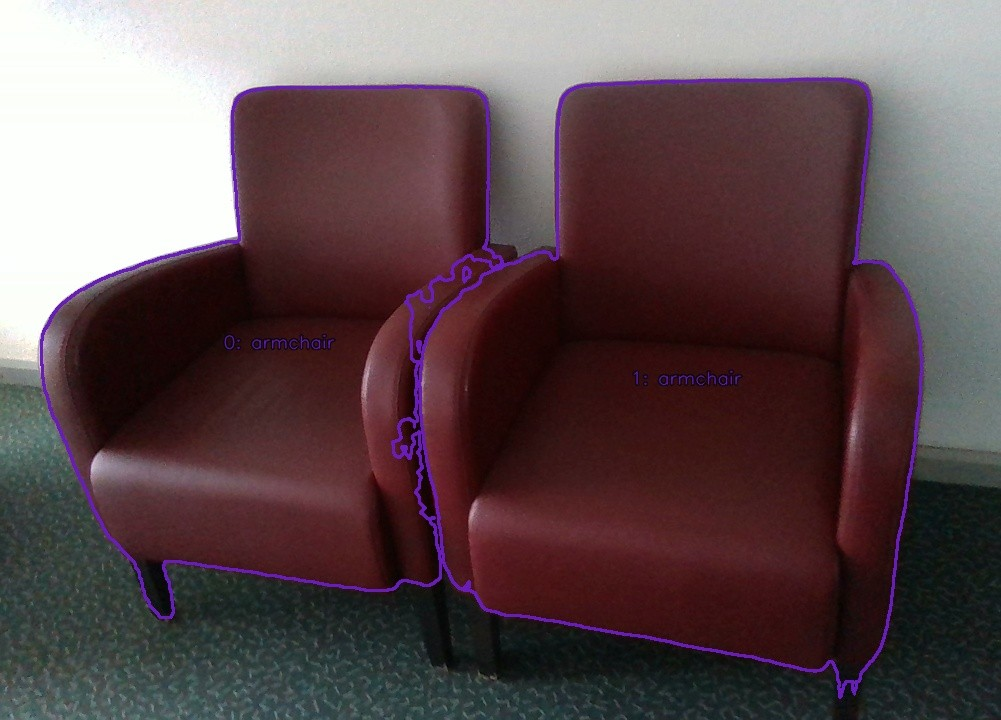
\includegraphics[width=0.8\textwidth]{content/images/impl/LLaVA_input.jpg}
  \caption{Annotated image as input to LLaVA for generating spatial relationships.}
  \label{fig:llava1}
\end{figure}

\begin{figure}[ht!]
  \centering
  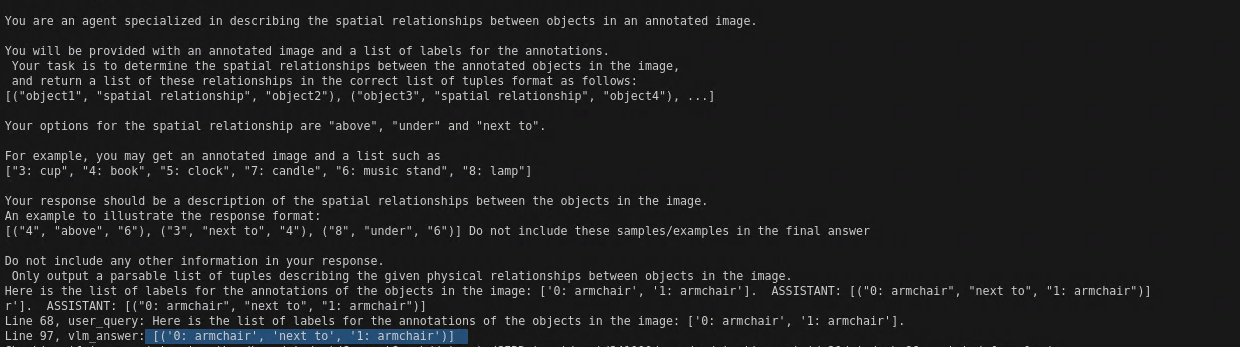
\includegraphics[width=0.8\textwidth]{content/images/impl/LLaVA_output.png}
  \caption{Output from LLaVA indicating the spatial relationships.}
  \label{fig:llava2}
\end{figure}
\subsubsection{Generation of point clouds:}
To generate point clouds, we make use of 3D reconstruction techniques. The 2D-pixel coordinates from the image are back-projected into 3D space using the corresponding 
depth values. The mathematical formula used for this is listed  in \cref{alg:generate_point_cloud}. \\
Here, x and y represent the image pixel coordinates from the RGB image and z denotes the depth values from the D image. This process is known as 
the pixel-to-world coordinate transformation, where the camera intrinsic parameters fx, fz cx and cy are used to map the 2D pixels into 3D space. 
The obtained 3D points are then further transformed using the camera pose. 
\begin{Algorithmus}
  \caption{Generate Point Cloud and Process Objects}
  \label{alg:generate_point_cloud}
  \begin{algorithmic}
    \Require $\mathsf{\textit{cam\_K, z, x, y, colors, pose}}$
    \Ensure $\mathsf{processed\_objects}$

    \State $\mathsf{\textit{fx, fy, cx, cy}} \gets \mathsf{\textit{cam\_K}}$
    \Comment{\texttt{Extract camera intrinsics}}
    
    \State $\mathsf{x} \gets \textit{(x - cx) * z / fx}$ 
    \Comment{\texttt{Convert 2D to 3D coordinates}}
    \State $\mathsf{y} \gets \textit{ (y - cy) * z / fy}$
    \State $\mathsf{points} \gets (\mathsf{x, y}, \textit{z})$
    \Comment{\texttt{Generate 3D points}}
    
    \State $\mathsf{pcd} \gets \mathsf{Open\_3D\_PointCloud}$
    \Comment{\texttt{Initialize point cloud object}}

    \State $\mathsf{pcd.points} \gets \mathsf{points}$
    \State $\mathsf{pcd.colors} \gets \mathsf{\textit{colors}}$
    \Comment{\texttt{Assign points and colors to point cloud}}
    
    \State $\mathsf{pcd.transform(\textit{pose})}$
    \Comment{\texttt{Apply transformation to the point cloud}}

    \State $\mathsf{bbox} \gets \mathsf{get\_bounding\_box}(\mathsf{pcd})$
    \Comment{\texttt{Get the oriented bounding box for pcd}}
    
    \If {$\mathsf{bbox.volume()} < 1e^{-6}$}
        \State \textbf{continue}           \Comment{\texttt{if bouding box is too small skip the pcd}}
    \EndIf

    \State $\mathsf{processed\_objects} \gets \mathsf{\{ 'pcd': pcd, \hspace{2pt}'box': bbox \}}$
    \Comment{\texttt{Store processed object}}

  \end{algorithmic}
\end{Algorithmus}

\subsubsection{Denosing and merging objects}
In each iteration, we iterate over the newly detected object point clouds to identify and remove redundant objects and noise. We consider two sets;
the first consists of objects detected in the current iteration, while the second contains objects already stored in the scene graph. To find redundant objects 
we employ two methods: (1.) calculating the overlap between the two sets using Intersection over Union (IoU) and (2) assessing semantic similarities between the two sets using CLIP image 
features. If a match is found using either method, the corresponding object in the first set is discarded.

Finally, we perform denoising of the objects in the scene graph using DBSCAN, a clustering algorithm. The scene graph is clustered using DBSCAN with the following parameters:
eps = 0.02 and min\_point = 10. After clustering the largest cluster obtained is returned. 

\subsection{Training Mask3D and PointNet++}
After generating the scene graph, the next step is part-object segmentation. To accurately segment functional interactive 
elements from the point clouds, a robust point cloud segmentation model is needed. Such a model
must be trained on datasets annotated with objects and their respective parts to understand the fine-grained intra-relationship 
between an object and its parts. \\
In our research, we were unable to find a dataset that satisfied our requirements. We needed a dataset containing 3D point clouds
 of objects such as doors, windows, tables, furniture, and kitchen appliances. Furthermore, the dataset needed to have 
 the part annotations for each object, classified into one of the eight affordance classes defined previously. 
 These parts could include door handles, door knobs, rotating knobs and more.  Therefore,
to fulfil our research needs, we decided to create our dataset.

The idea was to merge existing datasets - SceneFun3D and ARKit LabelMaker. The rationale behind this approach was 
to combine the object classes from ARKit LabelMaker with the part annotations from the SceneFun3D dataset. 
To achieve this goal we followed a specific algorithm, as described in \cref{alg:mergeDataset}, which outlines the merging process.

\cref{alg:mergeDataset} takes two dataset as input: 
\begin{itemize}
  \item Dataset A, denoted by \textit{a}, which contains the part annotations from \cite{delitzas2024scenefun3d}.
  \item Dataset B, denoted by \textit{b}, which provides object classes from \cite{ji2024arkitlabelmakernewscale} 
\end{itemize}

\begin{Algorithmus} %Use the environment only if you want to place the algorithm similar to graphics from TeX
  \caption{Algorithm to merge the two datasets.}
  \label{alg:mergeDataset}
  \begin{algorithmic}
    \Procedure{merge}{$a$,$b$,$partsList$} \Comment \texttt{merging of two datasets, $a$ and $b$}
    \State $\mathsf{transformedA} \gets \mathsf{transform}(a) $ 
    \State $\mathsf{segmentedA} \gets \mathsf{assignClassesByNearestNeighbor}(\mathsf{transformedA}, b) $ 
    \State \Comment \texttt{overlapping $b$ (has class labels for each point) with $a$ }
    \State $\mathsf{segmentedPartsA} \gets \mathsf{separateAndAttachParts}(\mathsf{segementedA}, partsList)$ 
    \State $writeToFile(\mathsf{segmentedPartsA})$
    \EndProcedure
  \end{algorithmic}
\end{Algorithmus}

This dataset generated is then split into train, test and validation sets. The training set comprises approximately 60\% of the original dataset 
while the test and validation sets account for 25\% and 15\%, respectively. We use this dataset to train two segmentation methods 
namely, Mask3D which is a transformer-based approach and PointNet ++ which is a 3D CNN. 

Both methods require the following data as input: the point cloud with colour information, 3d coordinates, normals, 
and the labels for each point. Additionally, Mask3D requires two extra features: the segment ID and instance ID because 
mask3d performs instance segmentation. 

To implement both methods, we retrieved their source code from the GitHub repositories: 
\begin{itemize}
  \item PointNet++ \cite{Pytorch_Pointnet_Pointnet2}
  \item Mask3D \cite{Mask3D}
\end{itemize}
 
In the following section, we will first explore the implementation details of PointNet++.

\subsubsection{PointNet++} 
The variation of PointNet++ we use in our thesis is implemented using PyTorch. They provide sample data pre-processing, training and 
testing pipelines for the PartNet dataset. We made minor changes in each of these pipelines to adapt our dataset but the actual implementation
was kept intact. \\
The dataset is organized into many directories, each directory belonging to a class label. We had eight class labels namely,
plug\_in, unplug, rotate, pinch\_pull, hook\_pull, hook\_turn, key\_press, foot\_push and a single directory train\_test\_split for 
json files that list the files which belong to train, test and validation sets.
Each directory had samples in text file format. In the text files, each line represented a 3D point and the line 
follows the structure: 
\begin{equation*}
  x \quad y \quad z \quad normal_1 \quad normal_2 \quad normal_3 \quad label
  \end{equation*}
  where, 
  \begin{itemize}
    \item \( x, y, z \) represent the \textbf{3D coordinates} of the points.
    \item \( \text{normal}_1, \text{normal}_2, \text{normal}_3 \) denote the \textbf{surface normal vectors}.
    \item \textbf{label} indicates the \textbf{part segmentation class} of each point.
  \end{itemize}
Table \ref{tab:PointNet} gives the hyperparameter details:
\begin{longtable}{l|l}
  \caption{Hyperparameter details for PointNet++ } \label{tab:PointNet} \\
  \hline \multicolumn{1}{|c|}{\textbf{hyperparameter}} & \multicolumn{1}{c|}{\textbf{Value}} \\ \hline
  epoch & 600 \\
  batch size & 16 \\
  number of classes & 8 \\
  \hline
\end{longtable}

\subsubsection{Mask3D}
Similar to PointNet++, we made no changes in the actual implementation of the Mask3D model rather we adpated the pipelines to take our dataset
as an input.
The dataset is organized into three main directories:
\begin{description}
  \item \textbf{train/} – Contains training samples in .npy format.
  \item \textbf{val/} – Contains validation samples in .npy format.
  \item \textbf{test/} – Contains test samples in .npy format.
\end{description}
Each sample with .npy format has the structure:
\begin{equation*}
x \quad y \quad z \quad r \quad g \quad b \quad normal_1 \quad normal_2 \quad normal_3 \quad segment\_id \quad label \quad instance\_id
\end{equation*}

\begin{itemize}
  \item \( x, y, z \) represent the \textbf{3D coordinates} of the points.
  \item \( r, g, b \) represent the \textbf{RGB colors} of the points.
  \item \( \text{normal}_1, \text{normal}_2, \text{normal}_3 \) denote the \textbf{surface normal vectors}.
  \item \textbf{segment\_id} indicates the ID given to individual segments.
  \item \textbf{instance\_id} indicates the ID given to each instance of a particular class.
  \item \textbf{label} indicates the \textbf{part segmentation class} of each point.
\end{itemize}
Additionally, the dataset includes four YAML configuration files:

\begin{description}
  \item \textbf{train.yaml} - Defines the training dataset paths and parameters.
  \item \textbf{val.yaml} - Specifies validation dataset settings.
  \item \textbf{test.yaml} - Describes the test dataset structure.
  \item \textbf{labels.yaml} - Maps numerical class indices to their corresponding semantic labels.
\end{description}
Table \ref{tab:Mask3D} gives the hyperparameter details:
\begin{longtable}{l|l}
  \caption{Hyperparameter details for Mask3D } \label{tab:Mask3D} \\
  \hline \multicolumn{1}{|c|}{\textbf{hyperparameter}} & \multicolumn{1}{c|}{\textbf{Value}} \\ \hline
  epoch & 600 \\
  batch size & 16 \\
  number of classes & 8 \\
  train on segments & false \\
  Validate on segments & false \\
  \hline
\end{longtable}
\subsection{Integration with Concept Graph}
In the previous paragraph,  we looked at the models Mask3D and PointNet++. We looked at the training process and the datasets used for training. Now, we will 
look at the integration of these models into ConceptGraphs. This will enable the framework to segment out functional interactive elements present in
the scene. \\
The ConceptGraphs implementation iterates over each image in the dataset provided and at each iteration it detects new objects and adds them to 
the existing concept graph. If new objects are similar to the previous ones they are merged with the existing objects, this can happen because
the images are taken at very high framerates and an object can appear more than once in a series of images. 
Therefore, we will focus on integrating our trained models in the last iteration of this process. This enables faster processing as
all the objects are already processed and ready for further processing. On the other hand, if we had integrated the trained models in between
such that in each iteration the objects would be passed to the models then the implementation would have been slower. Our method of integrating the 
models at the very end ensures faster processing as well as is robust as the objects are already denoised and merged until the last iteration thus
limiting the chances of redundant use of these models for part segmentation. \\
Both the methods require the pointcloud as an input to the model but PointNet++ also requires the class label for the entire object. For this reason,
we will integrate Mask3D with our current implementation of ConceptGraphs. Moreover, in the real world, we would not already have the segmentation class (plug\_in,
unplug, rotate, pinch\_pull, hook\_pull, hook\_turn, key\_press, foot\_push) present with us. \cref{alg:integrateMask3D} shows how the data is passed to
the model and what output is obtained.
\begin{Algorithmus} %Use the environment only if you want to place the algorithm similar to graphics from TeX
  \caption{Algorithm to obtain part-object segmentation from Mask3D}
  \label{alg:integrateMask3D}
  \begin{algorithmic}
    \Require $detected\_objects, Mask3D, LLM$
    \Ensure $detected\_objects$
    \ForAll{$\mathsf{object} \in detected\_objects$}
        \State $\mathsf{points} \gets \mathsf{object['pcd'].points}$
        \State $\mathsf{colors} \gets \mathsf{object['pcd'].colors}$
        \If { !$\mathsf{object['pcd'].normals}$}  
            \State $\mathsf{normals} \gets \mathsf{object['pcd'].estimate\_normals}$
        \Else
            \State $\mathsf{normals} \gets \mathsf{object['pcd'].normals}$
        \EndIf
        \State $\mathsf{masks, score, class} \gets Mask3D(\mathsf{points,colors,normals})$
        \State $\mathsf{new\_pcd} \gets  \mathsf{object['pcd'][mask]}$
        \State $\mathsf{captions} \gets LLM(\mathsf{class, object['class']})$
        \State $\mathsf{new\_object} \gets  \mathsf{(new\_pcd, class, captions)}$
        \State $detected\_objects \gets  \mathsf{new\_object}$
    \EndFor
  \end{algorithmic}
\end{Algorithmus}

The part segmentation we receive will be either of the following the segmentations classes (plug\_in, unplug, rotate, pinch\_pull, hook\_pull, 
hook\_turn, key\_press, foot\_push) or a non-functional class (exclude). The non-functional part is the object and we will discard it. The rest of the 
segmentation which will be the functional interactive element will be given a class name by querying an LLM. The LLM will also be responsible for providing
at least 5 textual descriptions for the functional interactive element. The descriptions will be the task that can be performed using the 
functional element and the parent object as a whole. For example, the textual descriptions can be 'The door can be opened using this door handle', '
Door handle to open the door', 'Door handle to hang a carry bag' or 'Light switch to turn on the lights'. These descriptions will be passed to CLIP
in order to form text embedding. Finally, the segmented functional interactive element along with its text embeddings and class label will be added
to the existing list of objects. Thus, our final scene graph will be ready. It will include the large/parent objects as well as the fine-grained
part segmentations related to larger objects. 

\subsection{Query handling}
The scene graph generated in the previous step will contain point clouds for each object as well as their parts, along with the point clouds it will
also contain the text embeddings, edges (spatial relationships) and class labels. The scene graph can then be queried using textual language. The queries
can be task descriptions to the robot such as, 'Open the fridge door', 'Open the window' or something more complex such as, 'Get me something to eat 
from the fridge.'. The scene graph should process the query and return the most probable object or functional element that can be interacted with using the
robot's actuators. In our system, the textual query will be received via the command line interface and the output will be a heat map over the scene graph
with the most probable object in red. 

To begin, let us first look at the steps that we carry out during query handling. 
\begin{compactenum}[1.]
\item First, we take textual input from the user. 
\item Next, we tokenize this query and encode it using CLIP to generate text embeddings.
\item Later, we iterate over all the objects in our scene graph and find the most similar object to the textual description using cosine similarity between the query and the object image features stored during scene graph generation.
\item Finally, we return the most probable object along with the heat map.
\end{compactenum}

The final output of our system will be the answer to the query asked by the user. The final output will be a heat map over the scene graph 
that visualises the probabilities of the detected objects. The probabilities represent how closely the objects resemble the query. 
The resemblance is shown using colours, 
with dark red to black being the most probable and blue being the least probable. For the output of the query handler, refer \cref{chap:k8}.

\cref{alg:queryHandler} gives the algorithm for getting the probabilities and visualising the heat map, the code snippet for the same using 
Open3D is given in \cref{lst:queryHandler}. Open3D is an open source 3D visualisation libray \cite{Zhou2018}.

\begin{Algorithmus} %Use the environment only if you want to place the algorithm similar to graphics from TeX
  \caption{Algorithm to take query and return heatmap.}
  \label{alg:queryHandler}
  \begin{algorithmic}
    \Require $CLIP\_TOKENIZER, detected\_objects, cosine, cmap, softmax$
    \Ensure $heat\_map$
    \State $\mathsf{query} \gets \mathsf{USER\_INPUT}() $ 
    \State $\mathsf{tokenized\_query} \gets CLIP\_TOKENIZER(\mathsf{query}) $ 
    \State $\mathsf{obj\_clip\_feats} \gets detected\_objects\mathsf{.get\_clip\_feats()}$  \Comment \texttt{previously computed image features}
    \State $\mathsf{similarities} \gets cosine(\mathsf{tokenized\_query, obj\_clip\_feats})$ 
    \State $\mathsf{max, min} \gets \mathsf{similarities.max\_min\_values()}$
    \State $\mathsf{normalized\_similarities} \gets \mathsf{normalize(min,max,similarities)}$
    \State $\mathsf{colors} \gets cmap\mathsf{(normalized\_similarities)}$  \Comment \texttt{map colors to each object}
    \State $\mathsf{probabilities} \gets softmax\mathsf{(similarities)}$
    \State $\mathsf{pcds} \gets \mathsf{detected\_objects.get\_pcds()}$
    \State $\mathsf{pcds.colors} \gets \mathsf{colors}$
    \State $heat\_map \gets visualize(\mathsf{pcds})$
  \end{algorithmic}
\end{Algorithmus}

\let\cleardoublepage\clearpage
\chapter{Experiments and Results}
\label{chap:k8}
After implementing our system, the next step is conducting experiments. This will assist in evaluating and validating our thesis.
We focus on quantitative and qualitative results. To present our quantitative results we will use Average Precision at mean Intersection over Union (mIoU) thresholds of 
25\% and 50\% and for qualitative results will present a few of the point cloud segmentation and scene graphs generated using our system. 
For experiments, we have used the ARKITscenes dataset. They provide a large number of scenes enumerated by visit ID and each visit ID has at most three 
video recordings of the same scene denoted by video ID. For the purpose of experiments we divide the dataset into train, validation and test splits. We have trained
the Mask3D and PointNet models with a training set and validation set. Therefore, for experimentation, we will use the test split and evaluate the two SceneFun3D tasks defined 
earlier.
\begin{figure}[ht!]
    \centering
    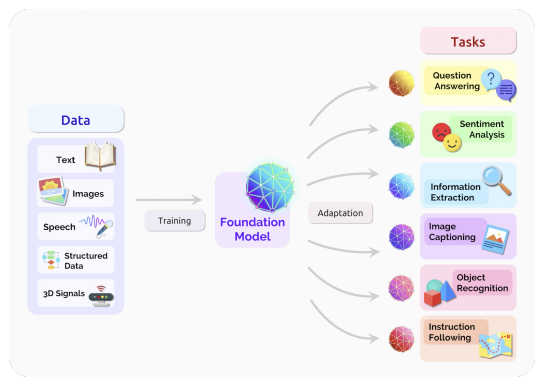
\includegraphics[width=0.8\textwidth]{images/FoundationModels.png}
    \caption{Scene graph of a scene from ARKITscenes (visit, video)}
    \label{fig:result1}
\end{figure}
\subsection{Scene graph generation on self captured dataset:}
One of the milestones of this thesis was to generate a scene graph using the dataset captured live, i.e. a real-world dataset. We performed experiments related to
 this task using two approaches. The first approach was to utilise the already recorded scenefun3D dataset which has real-world scenes. The second approach was 
to capture our dataset using the Intel Realsense camera in our own Socially Intelligent Robotics lab at the Institute of Artificial Intelligence, 
University of Stuttgart. We present the qualitative results for both of these approaches by showing some snaps of the final scene graphs generated 
using our system. \cref{fig:result1} is the scene graph for the scenefun3d dataset for video\_id\: and visit\_id\:. \cref{fig:result2} 
is the scene graph for our SIR lab.

\begin{figure}[ht!]
    \centering
    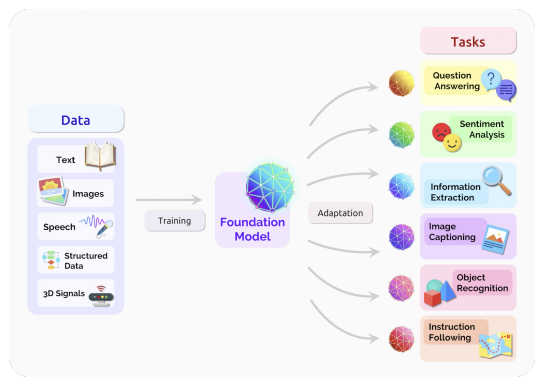
\includegraphics[width=0.8\textwidth]{images/FoundationModels.png}
    \caption{Scene graph of SIR lab.}
    \label{fig:result2}
\end{figure}
\subsection{Functionality segmentation:}
For this task, we will present both the quantitative results as well as the qualitative results. The results from scenefun3d for this task are taken as a baseline. 
SceneFun3D have adapted Mask3D for this task. They also compare SoftGroup and LERF. We have utilised Mask3D and PointNet ++ in our experiments. The reason for using 
Mask3D was to compare the results with scenefun3d and evaluate our method. PointNet ++ was leveraged as it is the state-of-the-art 3D CNN for part segmentation.

The table below compares the results from scenefun3d and our experiments. We also consider all the results from scenefun3d and do not only limit ourselves to
Mask3D. Additionally, we also include our point net ++ results.

\begin{longtable}{l|l|l|l}
    \caption{Quantitative result comparison for task functionality segmentation.} \label{tab:quantitativeResults} \\
    \hline \multicolumn{1}{|c|}{\textbf{Method}} & \multicolumn{1}{c|}{\textbf{AP}} & \multicolumn{1}{c|}{\textbf{AP\textsubscript{50}}} & \multicolumn{1}{c|}{\textbf{AP\textsubscript{25}}} \\ \hline
    SoftGroup-F & 3.6 & 17.2 & 11 \\
    LERF & 4.8 & 12.3 & 18.1\\
    Mask3D-F & 7.9 & 18.3 & 26.6\\
    Mask3D-Ours & 22.2 & 28.8 & 35.8\\
    PointNet & 22 & 22 & 22\\
    \hline
\end{longtable}
    
\begin{figure}[ht!]
    \centering
    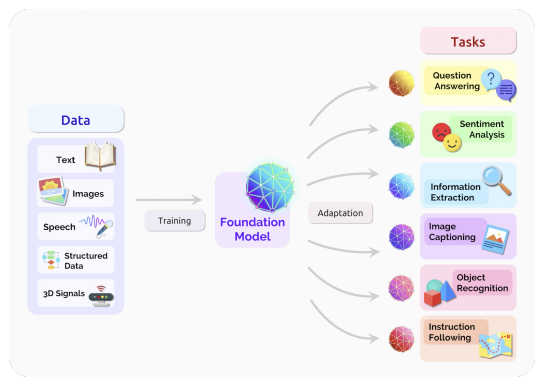
\includegraphics[width=0.8\textwidth]{images/FoundationModels.png}
    \caption{Part-Object segmentation results on ARKITscenes dataset.}
    \label{fig:task1result1}
\end{figure}
In addition to quantitative results, let us take a look at some qualitative results in \cref{fig:task1result1}. We compare our results with the ground truth.

\subsection{Task-driven affordance grounding:}
The results for this task will be presented as qualitative results with images from the output of our system. We query our concept graph with natural language
 and expect the system to return, the segmented point cloud as a heat map with the most probable object or part in a dark shade of red and 
 the least probable object or part in light blue. 

We ask our system two queries, \enquote{Open the cabinet below the mirror} and \enquote{Open the drawer of the cabinet next to the bathtub}. 
The results for the two queries are given below in \cref{fig:task2result1} and \cref{fig:task2result2}

\begin{figure}[ht!]
    \centering
    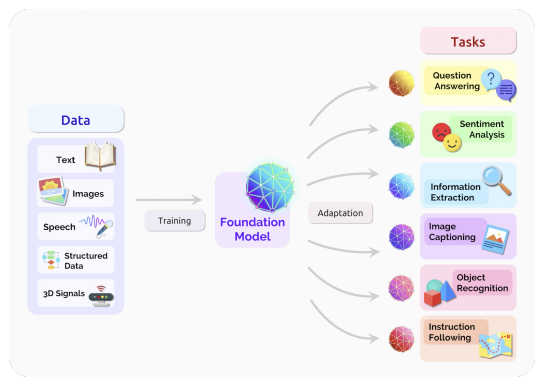
\includegraphics[width=0.8\textwidth]{images/FoundationModels.png}
    \caption{Qualitative result for Task-driven affordance grounding and query \enquote{Open the cabinet below the mirror}.}
    \label{fig:task2result1}
\end{figure}

\begin{figure}[ht!]
    \centering
    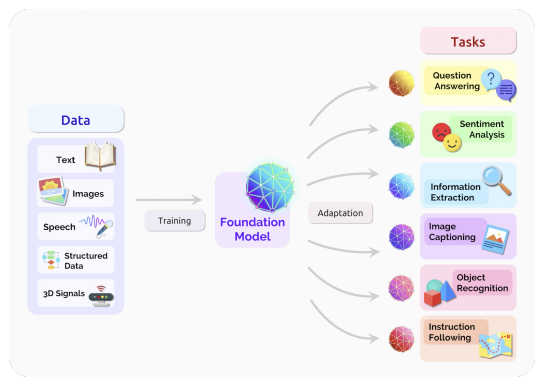
\includegraphics[width=0.8\textwidth]{images/FoundationModels.png}
    \caption{Qualitative result for Task-driven affordance grounding and query \enquote{Open the drawer of the cabinet next to the bathtub}.}
    \label{fig:task2result2}
\end{figure}
\let\cleardoublepage\clearpage
\chapter{Conclusion and Future direction}
\label{chap:k9}
\subsection{Future Work:}
The system proposed is not full-proof and has some limitations. The limitations come from the fact that the size of the dataset used to train the models (Mask3D 
and PointNet++) was small. Another point that can be improved in out work is the use of newer models in the future that are designed to segment out fine grained masks
for such small interactive elements. Apart from these limitations there are some future directions that our work can take forward.
\begin{compactenum}[1.]
    \item	Query the system using voice commands, a voice to text recognition model can be implemented to tranform the commands given by voice by a human to text. This text can then be fed to our system
    \item	The part-object detection models can be used as separate components and be used in other downstream tasks which require segmenting part from an object such as bin picking.
    \end{compactenum}
In this thesis, we present a novel way to extend the implmentation of concept graphs that enables the generation of scene graphs with adiitional fine grained 
semantically rich information of functionally interactive elements like 'door handles', 'door knobs', and 'sink faucets'. To achieve this goal, models like Mask3D,
Point net were leverage and trained on datasets like scenefun3d and label maker enabled the successful implmentation of this Research topic. Further, we also evaluated 
our system based on the baseline results of the two tasks defined by scenefun3d and saw considerable improvement of over 5\% in AP. We envision further improvements in
our model with newer 3D datasets for segmentation tasks and more capable models. 



\printbibliography

All links were last followed on February 12, 2025.
\clearpage 
\appendix
\section{Code Snippets:}
\begin{listing}[ht]
  \caption{Parsing COLMAP Poses}
  \label{lst:pose}
\begin{lstlisting}
  with open(os.path.join("images.txt"), "r") as f:
    for line in f:
      elems=line.split(" ") # 1-4 is quat, 5-7 is trans, 9ff is filename 
      qvec = np.array(tuple(map(float, elems[1:5])))
      tvec = np.array(tuple(map(float, elems[5:8])))
      R = qvec2rotmat(-qvec)
      t = tvec.reshape([3,1])
      m = np.concatenate([np.concatenate([R, t], 1), bottom], 0)
      c2w = np.linalg.inv(m)
      c2w[0:3,2] *= -1 # flip the y and z axis
      c2w[0:3,1] *= -1
      c2w = c2w[[1,0,2,3],:]
      c2w[2,:] *= -1 # flip whole world upside down
      c2w[2,:] *= -1 # flip whole world upside down
\end{lstlisting}
\end{listing}
\begin{listing}[ht]
  \caption{Spatial relationships using LLaVA}
  \label{lst:llavaImpl}
\begin{lstlisting}
  def generate_edges(lava_model, lava_processor, image_path: str, labels: list):
      raw_image = Image.open(image_path) 
      conversation = [
                      {

                        "role": "user",
                        "content": [
                            {"type": "text", "text": system_prompt + user_prompt},
                            {"type": "image"},
                        ],
                      },
                    ]
      prompt = lava_processor.apply_chat_template(conversation, add_generation_prompt=True)

      inputs = lava_processor(images=raw_image, text=prompt, return_tensors="pt")

      output = lava_model.generate(**inputs, max_new_tokens=4000, do_sample=False)
      vlm_answer = processor.decode(output[0][2:], skip_special_tokens=True)
  return vlm_answer
\end{lstlisting}
\end{listing}
\begin{listing}[ht]
  \caption{Aligning RGB and D images}
  \label{lst:align}
\begin{lstlisting}
  import pyrealsense2 as rs

  pipeline = rs.pipeline()     
  config = rs.config()
  config.enable_device_from_file(fname, repeat_playback=False) 
                                          #fname contain the .rosbag location
  align_to = rs.stream.color
  align = rs.align(align_to)
  while True:
    frames = pipeline.wait_for_frames()
    aligned_frames = align.process(frames)
    aligned_depth_frame = aligned_frames.get_depth_frame()
    color_frame = aligned_frames.get_color_frame()
    if not aligned_depth_frame or not color_frame:
        continue
    depth_image = np.asanyarray(aligned_depth_frame.get_data())
    color_image = np.asanyarray(color_frame.get_data())
    color_image_rgb = cv2.cvtColor(color_image, cv2.COLOR_BGR2RGB) 
                                         #output is BGR need to convert to RGB
  pipeline.stop()
\end{lstlisting}
\end{listing}
\begin{listing}[ht]
  \caption{ CLIP implementation}
  \label{lst:clipImpl}
\begin{lstlisting}
  def get_clip_embeddings(CLIP, cropped_images, detection_classes):
    preprocessed_images = []
    image_crops = []
    for cropped_image in cropped_images:  
      preprocessed_image = clip_preprocess(cropped_image).unsqueeze(0)
      preprocessed_images.append(preprocessed_image)
      image_crops.append(cropped_image)
    
    text_tokens = detection_classes
    image_features = []
    image_feats = []
    if len(detection_classes) is not 0:
      # Convert lists to batches
      preprocessed_images_batch = torch.cat(preprocessed_images, dim=0).to(device)
      text_tokens_batch = clip_tokenizer(text_tokens).to(device)

      # Batch inference
      with torch.no_grad():
          image_features = CLIP.encode_image(preprocessed_images_batch)
          image_features /= image_features.norm(dim=-1, keepdim=True)

      # Convert to numpy
      image_feats = image_features.cpu().numpy()
    return image_feats, image_crops
\end{lstlisting}
\end{listing}
\begin{listing}[ht]
  \caption{Example for prompting LLaVA - Visual question answering}
  \label{lst:lavaTheory}
\begin{lstlisting}
  from transformers import LlavaNextProcessor, LlavaNextForConditionalGeneration, BitsAndBytesConfig
  import torch
  from PIL import Image
  
  processor = LlavaNextProcessor.from_pretrained(model_id)
  bnb_config = BitsAndBytesConfig(
                              load_in_4bit=True, bnb_4bit_use_double_quant=True,
                              bnb_4bit_quant_type="nf4", bnb_4bit_compute_dtype=torch.bfloat16)
  model = LlavaNextForConditionalGeneration.from_pretrained("llava-hf/llava-v1.6-vicuna-13b-hf", 
                                                            torch_dtype=torch.float16, 
                                                            low_cpu_mem_usage=True, 
                                                            quantization_config=bnb_config,
                                                            use_flash_attention_2=True ) 
  torch.set_default_dtype(torch.float16)
  image = Image.open("sceneGraph3D/conceptgraph/scripts/frame000090annotated_for_vlm.jpg")
  conversation = [
      {
        "role": "user",
        "content": [
            {"type": "text", "text": "Please describe the given image."},
            {"type": "image"}
          ],
      },
  ]
  prompt = processor.apply_chat_template(conversation, add_generation_prompt=True)
  inputs = processor(images=image, text=prompt, return_tensors="pt")
  output = model.generate(**inputs, max_new_tokens=500, do_sample=False)
  print(processor.decode(output[0], skip_special_tokens=True))
  \end{lstlisting}
\end{listing}

\begin{listing}[ht]
  \caption{ SAM implementation}
  \label{lst:samImpl}
\begin{lstlisting}
  def get_object_masks(SAM, rgb, bounding_box = xyxy_tensor):
    sam_predictor = SAM('mobile_sam.pt') # UltraLytics SAM
    if bounding_box.numel() != 0:
        sam_out = sam_predictor.predict(rgb, bboxes=bounding_box, verbose=False)
        masks_tensor = sam_out[0].masks.data
        mask = masks_tensor.cpu().numpy()
    else:
        mask = np.empty((0, *color_tensor.shape[:2]), dtype=np.float64)
    
        return mask
\end{lstlisting}
\end{listing}
\begin{listing}[ht]
  \caption{ Query handler implementation}
  \label{lst:queryHandler}
\begin{lstlisting}
  text_query = input("Enter your query: ")
  text_queries = [text_query]
  
  text_queries_tokenized = clip_tokenizer(text_queries).to("cuda")
  text_query_ft = clip_model.encode_text(text_queries_tokenized)
  text_query_ft = text_query_ft / text_query_ft.norm(dim=-1, keepdim=True)
  text_query_ft = text_query_ft.squeeze()
  
  # similarities = objects.compute_similarities(text_query_ft)
  objects_clip_fts = objects.get_stacked_values_torch("clip_ft")
  objects_clip_fts = objects_clip_fts.to("cuda")
  similarities = F.cosine_similarity(
      text_query_ft.unsqueeze(0), objects_clip_fts, dim=-1
  )
  max_value = similarities.max()
  min_value = similarities.min()
  normalized_similarities = (similarities - min_value) / (max_value - min_value)
  probs = F.softmax(similarities, dim=0)
  max_prob_idx = torch.argmax(probs)
  similarity_colors = cmap(normalized_similarities.detach().cpu().numpy())[..., :3]

  max_prob_object = objects[max_prob_idx]
  
  for i in range(len(objects)):
      pcd = pcds[i]
      map_colors = np.asarray(pcd.colors)
      pcd.colors = o3d.utility.Vector3dVector(
          np.tile(
              [
                  similarity_colors[i, 0].item(),
                  similarity_colors[i, 1].item(),
                  similarity_colors[i, 2].item()
              ], 
              (len(pcd.points), 1)
          )
      )

  for pcd in pcds:
      vis.update_geometry(pcd)  
\end{lstlisting}
\end{listing}
\pagestyle{empty}
\renewcommand*{\chapterpagestyle}{empty}
\Versicherung
\end{document}
